%%
%% Preamble
%%
\documentclass[12pt,twoside]{mitthesis-manusdown}
\usepackage{lgrind}
%% These have been added at the request of the MIT Libraries, because
%% some PDF conversions mess up the ligatures.  -LB, 1/22/2014
\usepackage{cmap}
\usepackage[T1]{fontenc}
\pagestyle{plain}

% Packages are extensions to the basic LaTeX functions. Whatever you
% want to typeset, there is probably a package out there for it.
% Chemistry (chemtex), screenplays, you name it.
% Check out CTAN to see: http://www.ctan.org/
%%
\usepackage{graphicx,latexsym}
\usepackage{amsmath}
\usepackage{amssymb,amsthm}
\usepackage{longtable,booktabs,setspace}
\usepackage{chemarr} %% Useful for one reaction arrow, useless if you're not a chem major
\usepackage[hyphens]{url}
% Added by CII
\usepackage{hyperref}
\usepackage{lmodern}
\usepackage{float}
\floatplacement{figure}{H}
% End of CII addition
\usepackage{rotating}

% Next line commented out by CII
%%% \usepackage{natbib}
% Comment out the natbib line above and uncomment the following two lines to use the new
% biblatex-chicago style, for Chicago A. Also make some changes at the end where the
% bibliography is included.
%\usepackage{biblatex-chicago}
%\bibliography{thesis}


% Added by CII (Thanks, Hadley!)
% Use ref for internal links
\renewcommand{\hyperref}[2][???]{\autoref{#1}}
\def\chapterautorefname{Chapter}
\def\sectionautorefname{Section}
\def\subsectionautorefname{Subsection}
% End of CII addition

\hypersetup{
	colorlinks=true,
	linkcolor=blue,
	filecolor=blue,      
	urlcolor=blue,
}

% Added by CII
\usepackage{caption}
\captionsetup{width=5in}
% End of CII addition

% \usepackage{times} % other fonts are available like times, bookman, charter, palatino

% Syntax highlighting #22

% To pass between YAML and LaTeX the dollar signs are added by CII
\title{Statistically Inferring the Mechanisms of Phage-Host Interactions}
\author{Joy Yang}
% The month and year that you submit your FINAL draft TO THE LIBRARY (May or December)
\thesisdate{March 22, 2019}
\degreemonth{June}
\degreeyear{2019}

\prevdegrees{B.A., Statistics, University of California, Berkeley (2011)}

\supervisor{Martin Polz}{Professor, Civil \& Environmental Engineering}
\degree{Doctor of Philosophy}
%If you have two advisors for some reason, you can use the following
% Uncommented out by CII
% End of CII addition
\chairman{Christopher Burge}{Director, Computational and Systems Biology Graduate Program}
\committeeone{David Bartel}{Chairman, Thesis Committee}{Professor of Biology}
\committeetwo{Jeff Gore}{Member, Thesis Committee}{Associate Professor of Physics}
\committeethree{Libusha Kelly}{Thesis Supervisor/External Member, Thesis Committee}{Assistant Professor, Albert Einstein College of Medicine}

%%% Remember to use the correct department!
\department{Program in Computational and Systems Biology}
% if you're writing a thesis in an interdisciplinary major,
% uncomment the line below and change the text as appropriate.
% check the Senior Handbook if unsure.
%\thedivisionof{The Established Interdisciplinary Committee for}
% if you want the approval page to say "Approved for the Committee",
% uncomment the next line
%\approvedforthe{Committee}


% Added by CII
%%% Copied from knitr
%% maxwidth is the original width if it's less than linewidth
%% otherwise use linewidth (to make sure the graphics do not exceed the margin)
\makeatletter
\def\maxwidth{ %
  \ifdim\Gin@nat@width>\linewidth
    \linewidth
  \else
    \Gin@nat@width
  \fi
}
\makeatother

\renewcommand{\contentsname}{Table of Contents}
% End of CII addition

\setlength{\parskip}{0pt}

% Added by CII

\providecommand{\tightlist}{%
  \setlength{\itemsep}{0pt}\setlength{\parskip}{0pt}}

\Acknowledgements{

}

\Dedication{

}

\Preface{

}

\Abstract{
Bacteriophage and their hosts are locked in an age-old arms race.
Successful bacteria are subject to predation, forcing the population to
diversify, and phage are also quick to adapt tactics for infecting these
potential hosts. Sampling of closely related bacterial strains that
differ in phage infection profiles can further elucidate the mechanisms
of infection. The Polz Lab maintains the Nahant Collection - 243 Vibrio
strains challenged by 241 unique phage, all with sequenced genomes. This
is the largest phylogenetically resolved host-range cross test available
to date. Genetically mapping out the depths of this dataset requires
carefully designed analysis techniques as well as further experimental
exploration.

First, we narrow in on a specific phage in the Nahant Collection,
2.275.O, to \emph{characterize the pressures that may select for phage
that shuttle their own translational machinery}. While translation is
generally considered a hallmark of cellular life, some phage carry
abundant tRNA. 2.275.O carries 18 tRNA spanning 13 amino acids. We find
that while encoding translation-related components requires shuttling a
larger phage genome, it also reduces dependence on host translational
machinery, allowing the phage to be more aggressive in degrading and
recycling the host genome and other resources required for replication.

Next we \emph{develop a systematic approach for uncovering genomic
features that underlie phage-host interactions}. We find that correcting
for phylogenetic relationships allows us to pick out relevant signals
that would otherwise be drowned out by spurious correlations resulting
from statistically oversampled blooms of microbes. Using these results,
we wrote an interative javascript visualization to facilitate the
process of developing testable hypotheses concerning the mechanisms of
phage infection and host response. From the visualization, we are able
to identify, in the hosts, mobile genetic elements containing
restriction modification systems that may defend against infection, as
well as membrane protein modifications that may serve as phage
attachment sites.
}

	\usepackage{tikz} \usetikzlibrary{arrows}
\usetikzlibrary{decorations.pathreplacing} \usetikzlibrary{shapes}
% End of CII addition
%%
%% End Preamble
%%
%
\begin{document}


\pagestyle{plain}
% Everything below added by CII
  \maketitle
\begin{abstract}
	Bacteriophage and their hosts are locked in an age-old arms race.
Successful bacteria are subject to predation, forcing the population to
diversify, and phage are also quick to adapt tactics for infecting these
potential hosts. Sampling of closely related bacterial strains that
differ in phage infection profiles can further elucidate the mechanisms
of infection. The Polz Lab maintains the Nahant Collection - 243 Vibrio
strains challenged by 241 unique phage, all with sequenced genomes. This
is the largest phylogenetically resolved host-range cross test available
to date. Genetically mapping out the depths of this dataset requires
carefully designed analysis techniques as well as further experimental
exploration.

First, we narrow in on a specific phage in the Nahant Collection,
2.275.O, to \emph{characterize the pressures that may select for phage
that shuttle their own translational machinery}. While translation is
generally considered a hallmark of cellular life, some phage carry
abundant tRNA. 2.275.O carries 18 tRNA spanning 13 amino acids. We find
that while encoding translation-related components requires shuttling a
larger phage genome, it also reduces dependence on host translational
machinery, allowing the phage to be more aggressive in degrading and
recycling the host genome and other resources required for replication.

Next we \emph{develop a systematic approach for uncovering genomic
features that underlie phage-host interactions}. We find that correcting
for phylogenetic relationships allows us to pick out relevant signals
that would otherwise be drowned out by spurious correlations resulting
from statistically oversampled blooms of microbes. Using these results,
we wrote an interative javascript visualization to facilitate the
process of developing testable hypotheses concerning the mechanisms of
phage infection and host response. From the visualization, we are able
to identify, in the hosts, mobile genetic elements containing
restriction modification systems that may defend against infection, as
well as membrane protein modifications that may serve as phage
attachment sites.
\end{abstract}


  \hypersetup{linkcolor=black}
  \setcounter{tocdepth}{2}
  \tableofcontents


  \listoffigures


\raggedbottom

\chapter*{Acknowledgements}\label{acknowledgements}
\addcontentsline{toc}{chapter}{Acknowledgements}
\begin{center}\includegraphics[width=0.85\linewidth]{figuresintro/emonephage} \end{center}
\begin{quote}
``One Christmas Tukey gave his students books of crossword puzzles as
presents. Upon examining the books the students found that Tukey had
removed the puzzle answers and had replaced them with words of the
sense: `Doing statistics is like doing crosswords except that one cannot
know for sure whether one has found the solution.'\,'' - David
Brillinger {[}1{]}
\end{quote}
At some point during our many meetings, my advisor Martin looked at me
and said, ``well, I suppose it takes a village.'' This statement sums up
my graduate experience very concisely, and I'll now proceed to ramble on
about the village that was kind enough to support me throughout graduate
school.

First, as already mentioned, my advisor, Martin Polz, who has been
incredibly patient with me, allowing me the freedom to learn anything I
felt an impulse to learn. And while at first he very rarely discouraged
going down new paths, he became quick to warn me against rabbit holes
when he realized my inability to avoid them. His uncanny insights often
lead me to wonder whether he had known and was hiding the answers all
along.

My co-advisor Libusha Kelly is always willing to provide feedback on
everything I write, however hopeless or trivial the draft may be. She
has been thoughful and dedicated in making trips from New York in order
to attend my committee meetings in person. And I very much appreciate
her ability to ask just the right questions whenever I lack the capacity
for words.

The Computational Sciences Graduate Fellowship through the Department of
Energy supported me financially during four years of my PhD, and
provided me with funding for workstations, conferences, and professional
development. I am incredibly grateful for their support. Their
``requirements,'' which I like to think of as perks held me to the
promises I made to them and to myself upon first starting graduate
school.

I have been incredibly lucky to have benefitted from starting my PhD
following the heroic efforts of Kathryn Kauffman in carefully assembling
and archiving the Nahant Collection. Working with this dataset and the
organisms themselves has been an amazing avenue for me to synthesize and
process what I'd studied in books and classes. I'm grateful to Fatima
Hussain for having taught me to grow phage, Joseph Elshirbini for having
introduced me to the joys and headaches of javascript, Javier Dubert for
showing me how to transform \emph{Vibrio}, Dave VanInsberghe for
rescuing me from my NCBI submission woes, Annie Yu for being a partner
in crime during all the late night experiments, Fabiola Miranda for
allowing me to use her reagents whenever I'm unprepared myself, and
Bruno Janeiro, Clovis Borges, Hannah Gavin, Manoshi Datta, Nate Cermak,
Phil Arevalo, Alison Takemura, Diana Chien, Christopher Corzett, plus
anyone who I've failed to mention in the Polz lab for all the serious
scientific discussions as well as the occasional banter.

My committee, all having students of their own to advise, has been
generous in donating many hours of their time toward ensuring that I had
all the resources I needed to proceed. After seeing that I had an
interest in tRNA, and knowing of my utter incapacity for working with
RNA at the bench, David Bartel introduced me to a post-doctoral fellow
in his lab, Wenwen Fang. I am very grateful toward Wenwen, without whom
the entirety of Chapter 2 would not have been possible. Despite having
witnessed my denseness as a student in his class, Jeff Gore agreed to
serve on my committee and has provided me with incredible scientific,
career, and life advice. I learned through working with Philippe
Rigollet that, even if I'm entirely intimidated, it's much better to ask
questions in person when I don't understand than to spend many emails
trying to type math into paragraphs while trying to implement the
algorithm we'd discussed - which he was patient enough to bear with me
through. I would also like to thank Philippe's students, especially JC
Hütter, for help with brainstorming statistical methods and checking my
calculations.

Additionally, Bruce Tidor suffered through not one, but two qualifying
exams with me. Eric Alm provided me with a stimulating environment to
work in during my first two years; I am lucky to have overlapped with
many brilliant people there whose support and encouragement I deeply
appreciate. Chris Burge has been a calm and collected voice of reason
for our entire graduate program, and I am thankful for his guidance
during the roughest moments of my PhD.

As teaching truly is the best way to learn, I'm very appreciative of
Aviv Regev and Piyush Gupta's willingness to allow my co-TA Jonathan Teo
and I to experiment with new homework problems and different ways of
teaching recitation. I learned so much from Caroline Uhler and Stefanie
Jegelka, as well as from my co-TAs Jennifer Tang, Abigail Katkoff, and
Tahin Syed. I'm also very thankful to all of the students, who I've
served as a TA to, for allowing me to learn with them.

While I won't rattle off all of my teachers since preschool, I am
certaintly grateful to every one of my teachers since preschool. Thank
you especially to the teachers who had the patience and ingenuity to
teach each topic using three to five different approaches.

I would like to thank Yihui Xie for
\href{https://github.com/rstudio/bookdown}{bookdown}, Chester Ismay for
\href{https://github.com/ismayc/thesisdown}{thesisdown}, and maintainers
of all their dependencies (including R and latex) for making these tools
freely available. If these thanks seem out of place, I assure you they
are not, it has been exhilarating and of enormous convenience to have
been able to integrate code into this thesis easily.
\begin{center}\includegraphics[width=0.7\linewidth]{figuresintro/bacmanSmall} \end{center}

As for all of the social support I've been blessed with, I will mention
the groups but refrain from listing individual names due to a preference
for privacy. I hope it is nevertheless clear how much I appreciate
everyone, and I hope this does not offend anyone who I do not list by
name.

The Parsons Laboratory has been a great place for learning about
environmental sciences, as well as for making what I feel will be
life-long friends. I can't imagine going through graduate school without
this wonderful community.

The Computational and Systems Biology graduate students is such a fun
group of fascinated and fascinating individuals. I've enjoyed studying,
joking about hypothetical science, and wandering the ``back-alleys'' of
Kennebunkport together. Jacquie Carota is an incredible individiual,
thank you for making sure that we stay afloat.

Through the Computational Sciences Graduate Fellowship, I've met so many
people from all over the US in various disciplines, all excited about
computing. I feel very lucky to have been able to share science and
shenigans with everyone when we meet each year.

My amazingly generous classmates have spent many hours reviewing
difficult concepts, entertaining philosophical discussions, and doing
countless rounds of resume revisions with me. Thank you, I can only hope
to send forward all the good karma.

For all of the roommates that I've lived with, thank you for tolerating
me. My first year roommate fed me and dragged me home when I was still
acclimating to graduate school and barely able to function. During my
second and third years, I felt that I'd truly found a home in 22 Mag,
and this is entirely due to the warmth and generosity of my roommates. I
am amazed that we'd turned our pantry into a lab. And as for 77, where I
landed after signing a roommate agreement littered with hidden white
text, I still suspect that everyone is in on the long con. Beyond all
the craziness of shoving trees out the window and throwing pumpkins off
the roof, you're my people and I care about you.

I must also mention all my Bears who've supported me beyond college and
has made an effort to keep in touch through assembling the most
socially-conscious and depressing book club fathomable; a fantasy
football league, where the only currency exchanged is embarassment; and
superbowl squares, when regardless of where everyone is living, we all
participate in a gif exchange.

After quizzing one of his students, Tukey purportedly thought for a
while and said ``Well, what I think you need is folk dancing.'' I would
like to thank everyone above for folk dancing with me. Without all of
you, I would not feel human.

And finally, I would like to thank my family. My grandparents, Yang Su
Hua, Yang Xiang Wu, Zhao Rui Fang, and Dai Yong Nian for their
incredible strength and wisdom. And my parents, Aiping Dai and Dan Yang,
for endless advice, asked and unasked for. I am grateful for their
unconditional love and support, and for having placed me in an
environment where I never needed to worry about basic needs or survival
instincts, and so, had the freedom to develop a love for learning.

\chapter{Introduction}\label{introduction}

There are approximately 10 million viral particles per milliliter of sea
water {[}2{]}. At such numbers, these tiny 30-100 \(nm\) particles can
have an enormous impact on the ecosystem. To illustrate with a
particularly stunning example, \emph{Emiliana huxleyi} (a marine algae)
can bloom to 1-100 thousand cells per mL over an area of 250,000
\(km^2\) (in the upper 200 \(m\) of the ocean) {[}3{]}. After only a
week, these blooms collapse, releasing calcite into the seabed and
cloud-forming dimethyl sulfide into the atmosphere. This population
collapse is largely attributed to predation by coccolithoviruses {[}4,
5{]}.

The most common viruses are bacteriophage. These viruses' hosts
(bacteria) are also abundant, at around 1 million cells per milliliter
of sea water. This means ``rare'' events can happen frequently. For
example, in order for a successful lytic infection to occur, a phage
must encounter a bacterial host whose cell surface proteins it can bind
to, protect itself from the host restriction modification systems, and
replicate within its hosts cellular environment. All these road blocks
make successful lytic infections rare {[}6{]}; however there are
approximately 36 million \(km^3\) of water in the top 100m of the sea.
Therefore, rare events for a single cell do not equate to rare events
for the whole population {[}7{]}. In fact, it has been estimated that
new viruses are produced at rates of 1 million to 10 million particles
per milliliter per hour {[}8{]}. From this, assuming an average burst
size of 50 viruses per lytic event, the number of infections initiated
by phage per second somewhere in the ocean can be very roughly
approximated to be on the order of Avagadro's number {[}9{]}. \newline
\begin{figure}[tb!]

{\centering \includegraphics[width=0.5\linewidth]{figuresintro/coccolithophores} 

}

\caption{\label{fig:coccolithophores}Emiliania huxleyi population collapse within a week of the bloom (bloom depicted here, image from NASA Earth Observatory) is largely attributed to predation by coccolithoviruses.}\label{fig:coccolithophores}
\end{figure}
Lytic infections select for resistant hosts, forcing the population to
diversify, and resistant hosts select for compatible phage variants.
This rapid, recursive evolutionary arms race occuring at such a large
scale leads to highly diverse phage. The recent explosion in
bacteriophage genomes has revealed that phage genomes are highly mosaic
in structure {[}10{]}, suggesting frequent recombination; and contain
hoards of uncharacterized proteins. On average, approximately 70\% of
open reading frames in a phage are unannotated hypothetical proteins
{[}11{]}. While perplexing, this vast unknown may hold exciting
prospects for future research.

\section{Background on phage research, focusing on one-step
growth}\label{background-on-phage-research-focusing-on-one-step-growth}

Bacteriophage were discovered in 1915 by Frederick Twort then
independently again in 1917 by Felix d'Herelle. These ``anti-microbes''
were first studied for their potential to treat bacterial infections,
but this interest declined in the 1930s due to the success of
antibiotics. However, bacteriophage research quickly became foundational
to molecular genetics {[}12, 13{]}, as their small genomes, rapid growth
rate, and low-maintenance nature make them particularly convenient for
experimentation. In fact, many of the insights into the nature of DNA
came out of ``the phage group,'' an informal network of researchers
centered around Max Delbrück, who, starting in 1945, taught an annual
phage course in Cold Spring Harbor {[}14{]}. For example, in 1943,
Salvador Luria and Max Delbrück showed using T1, the (lack of) Poisson
distribution, and jackpotting that mutations occur spontaneously and can
be selected for, as opposed to being induced by a selection event
{[}15{]}. In 1952, using the T2 phage and a Waring blender, Alfred
Hershey and Martha Chase showed that it is DNA, and not protein, that
encoded the genetic material {[}16{]}. In 1957, Seymour Benzer showed
using T4's rII gene that recombination occurs on the nucleotide level
{[}17, 18{]}. In 1961, Crick, et al. showed, using Benzer's T4 rII
system and various combinations of double and triple frameshift
mutations, that the genetic code consists of triplet bases {[}19{]}. We
will next outline in greater detail a particular study, the Ellis and
Delbrück one-step growth experiment. As one of the earliest ``phage
group'' studies, it laid out the experimental framework for others to
come. Much of this framework is still widely used today; and in fact,
for the purposes of this thesis, the following background may help
clarify the methodological details presented in Chapter 2.

The Ellis-Delbrück study marks the introduction of Max Delbrück to
bacteriophage research {[}20{]}. In the mid-1930s, Emory Ellis was an
analytical chemist at Cal Tech working in cancer research. He had been
drawn to cancers induced by viruses, such as the Rous sarcoma virus and
the Shope rabbit papilloma virus; however, as so little was known about
viruses at the time, he decided that a fundamental understanding of
their biology was necessary in order to proceed. So he chose to start
with bacterial viruses (as opposed to mammalian viruses or plant
viruses) for the practical considerations of time, space, and cost. At
the time, however, the most commonly accepted view, championed by Jules
Bordet and John Northrop, was that the bacterial lysis witnessed by
d'Herelle had been incorrectly interpretted as an infection by an
exogenous body, when it was actually an endogenously catalyzed lytic
event. Ellis's goal was therefore to replicate d'Herelle's studies by
first isolating a virus for \emph{E. coli} from sewage (as he had a
culture of \emph{E. coli} gifted to him by a colleague), then
reproducing the stepwise pattern of phage growth.

Max Delbrück, on the other hand, had studied theoretical physics. And
influenced by Niels Bohr, he ventured into biophysics, where he became
interested in characterizing the nature of the gene. Eventually,
Delbrück arrived at Caltech to work on Drosophila genetics, but quickly
became frustrated. Instead, he developed an interest in viruses and
bacteriophage, thinking that ``the growth of phage was essentially the
same process as the growth of viruses and the reproduction of the
gene.'' So he sought out Ellis, and the two began to collaborate. The
above biographical details of Ellis and Delbrück's work together is
summarized from William Summers' \emph{How Bacteriophage Came to Be Used
by the Phage Group} {[}20{]}.
\begin{figure}[tb!]

{\centering \includegraphics[width=0.7\linewidth]{figuresintro/oneStepGrowth} 

}

\caption{\label{fig:onestepgrowth}By synchronizing infection assaying phage concentration at short, approximately 10 minute, time intervals, Ellis was able to see that phage growth appears to occur in bursts. The y-axis shows P/P0 in log-scale. P0 is the initial concentration of plaque forming units, and P is the concentration at a particular time. This image is from their original paper, \textcopyright 1939, by The Rockefeller Institute for Medical Research, adapted under \href{http://creativecommons.org/licenses/by-nc-sa/4.0/}{CC BY-NC-SA 4.0}}\label{fig:onestepgrowth}
\end{figure}
The Ellis-Delbrück paper {[}21{]} combines the work that Ellis had been
doing on phage growth curves with Delbrück's characterization of the
statistical nature of infections, which has, over time, evolved into the
statistics of what is now known as the multiplicity of infection (MOI,
or, the ratio of phage particles to bacterial cells).

The setup of Ellis's one-step growth experiment was simple. Essentially,
the idea was to synchronize at least the first round of infection in the
following way:
\begin{enumerate}
\def\labelenumi{\arabic{enumi}.}
\item
  Mix bacteria and viruses at a high concentration (on the order of
  \(10^9\) bacteria and viruses per mL), allow 5 minutes for the viruses
  to adsorb onto their hosts.
\item
  Dilute this mixture thoroughly using growth media (at a 1:12,500
  ratio) so that additional adsorption is unlikely to occur.
\item
  At approximately 5 minute intervals, plate samples of equal volume of
  this dilution on a background of concentrated bacteria in order to
  count how many viral particles had formed.
\end{enumerate}
From this type of growth curve, it is possible to deduce the latent
period, or the amount of time a phage spends replicating within a cell
before the progeny lyse the cell; as well as the burst size, or the
number of phage progeny that are produced from each infection.

Delbrück's statistical characterization of phage infections was equally
intuitive. When there is a uniform probability for an event to occur in
time or space, the number of events that occur in a given interval of
time or section of space follows a Poisson distribution. A few concrete
examples of events that can be modelled using a Poisson distribution
include the number of yeast cells in each batch of Guinness beer
(courtesy W.S. Gosset, or ``Student,'' of the Student's T-test)
{[}22{]}, the number of phone calls arriving at a call center within a
minute (A. K. Erlang), or the number bombs that fall in regions of
London during World War II (R. D. Clarke) {[}23{]}. Analogous to these
examples is the number of bacteriophage present in a given volume of
liquid. In particular, the probability of seeing \(k\) phage in a
milliliter is \[P( X = k ) = \frac{ \lambda^k e^{-\lambda} }{ k! }\]
where \(\lambda\), the rate parameter, is the average number of phage
present in each milliliter.
\begin{figure}[tb!]

{\centering \includegraphics[width=1\linewidth]{figuresintro/poissonThresholded} 

}

\caption{\label{fig:poisson}On the left is a picture of a phage plaque assay on a petri dish. The light hazy layer in the picture is a "lawn" of bacteria, and the spots scattered on top are "clearings" or "plaques." These plaques each can roughly be thought of as having grown out of one infection. The plaque count should then be proportional to the concentration of phage used for the plaque assay. On the right, a poisson distribution describes counts of an event in fixed intervals when there is a uniform probability for occurrence over the entire space. Phage dispersal on a plate is roughly uniform, and so plaque counts on equal areas should follow a Poisson distribution. The image analysis above was done with freshman miniUROPs Madelyn Focaracci and Jessica Wang. A timelapse plate read is also available online: \href{https://youtu.be/93p5phFAuo0}{https://youtu.be/93p5phFAuo0}.}\label{fig:poisson}
\end{figure}
One way to infer this parameter is to simply take the average - after
making multiple plates of one milliliter aliquots of the same sample,
count the number of plaques (or infection clearnings) on each plate, and
divide this by the number of plates. This is, in fact the maximum
likelihood estimate,
\(\hat{\lambda}_{MLE} = \frac{1}{n} \sum_{i=1}^{N} k_i\).

Delbrück suggested another way to infer this parameter - according to
the Poisson distribution, the fraction of plates without plaques is
expected to be
\[P( X = 0 ) = \frac{ \lambda^0 e^{-\lambda} }{ 0! } = e^{-\lambda}\]
The rate parameter can then also be estimated as
\(\hat{\lambda}_0 = -log(\frac{N_0}{N})\), where \(N_0\) is the number
of plates without any plaques.

Ellis and Delbrück observed, however, that there was consistently a
discrepancy between the two estimates. The second was almost three times
higher than the first (in their paper, \(\hat{\lambda}_{MLE} = 0.22\),
while \(\hat{\lambda}_0 = 0.56\)). This lead them to conclude that there
may not always be a direct correspondence between phage particles and
plaques\footnote{Because the title of this thesis includes the word
  ``statistical,'' there is some pressure to be statistically precise.
  So to be fair, the second estimate,
  \(\hat{\lambda}_0 = -log(\frac{N_0}{N})\) is a biased estimate of
  \(\lambda\). \(N_0 \sim Binomial(p_0, N)\), where
  \(p_0 = e^{-\lambda}\). Using a Taylor expansion around \(p_0 N\), we
  see that
  \(E(log N_0) = log(p_0 N) - \frac{1-p_0}{2p_0 N} + O(1/N^2)\).
  Therefore,
  \(E(\hat{\lambda}_0) = \lambda +\frac{1-p_0}{2p_0 N}+O(1/N^2)\). This
  calculation can be verified by plugging in values of \(N\) and
  \(\lambda\) and either running simulations or taking the sums. Given
  Ellis and Delbrück's experimental setup, this bias is small. Forty
  plates were tested, and if we assume the true rate parameter was 0.22,
  the first order bias term is 0.003, which doesn't come close to the
  discrepancy observed. Their conclusions are, therefore, still
  well-founded.}. The comparison of these two estimates was termed the
``efficiency of plating.''

The efficiency of plating is not a very commonly reported statistic
today, perhaps because the biological meaning of this statistic is
somewhat opaque. However, the application of the Poisson distribution
toward approximating phage infections has been adapted slightly and is
now still commonly used to design experiments. To elaborate, if we
assume that all plaque-forming phage are able to find a host, then the
bacterial cells themselves are now analogous to the milliliter aliquots
from the description above. The number of phage infecting each bacteria
follows a Poisson distribution, with the rate parameter being the
multiplicity of infection (MOI), or the ratio of phage particles to
bacterial cells. The proportion of uninfected bacterial cells (infected
by 0 phage) can be expected to be \(P(Y = 0) = e^{-\lambda_{MOI}}\), the
proportion of bacterial cells infected by just 1 phage can be expected
to be \(P(Y = 1) = \lambda_{MOI} e^{-\lambda_{MOI}}\), and the
proportion of multiple infections, or bacterial cells infected by more
than one phage, can be expected to be
\(P(Y > 1) = 1-(1+\lambda_{MOI})e^{-\lambda_{MOI}}\). For phage-host
pairs where infection by more than one phage results in a different
infection phenotype than infection by just one phage, it may be of
interest to the experimenter to pick a low MOI, tuning \(P(Y > 1)\) in
order to control the number of multiple infections. For experiments
where the goal is to observe a signal during infection, for example, RNA
sequencing looking for changes in host gene expression during infection
(as is the case in Chapter 2 of this thesis), it may be of interest to
the experimenter to pick a high MOI, tuning \(P(Y=0)\) in order to
reduce the background signal from uninfected cells.

Returning to the Ellis-Delbrück paper, the authors go on to describe
many additional carefully executed experiments, which will not be
further described here. However, to summarize a few highlights, they
were able to conclude that plaque counts correlate incredibly well with
phage concentration, and so each plaque likely grew from one instance of
infection; during the growth experiment, phage concentration increases
in a stepwise manner, indicating that phage are produced in bursts; and
phage growth depends on bacterial growth. Recalling their original goal
of assessing whether the bacterial death witnessed by d'Herelle was the
result of endogenous enzymatic lysis or killing by an obligate
intracellular parasite, they concluded that, while it is possible a
different type of phage exists, theirs was an obligate intracellular
parasite. This main conclusion is important as it laid the foundations
for other studies based in phage. Additionally, their study also has
lasting methodological impacts. In particular, Ellis's one step growth
curve continues to be the most accurate method for measuring the latent
period and burst size for a phage-host pair, and Delbrück's application
of the Poisson distribution to infection frequencies is widely used for
selecting an MOI during the design of experiments. Chapter 2 of this
thesis, which explores the action of phage tRNAs during infection,
extensively utilizes both of these methodological techniques.

\section{Phage research today, in the era of
sequencing}\label{phage-research-today-in-the-era-of-sequencing}

In 1944, Delbrück had drafted a ``phage treaty,'' in which he urged his
colleagues to focus their attention on the T-phages (T1, T2,\ldots{},
T6). Because of this, the T-phages became incredibly well characterized
model organisms. Bacteriophage research today, is often of a different
flavor. While a concerted effort is valuable, studying model organisms
comes with limitations, as our actual environment is much more diverse.
And conveniently, sequencing costs have been declining, according to the
National Human Genome Research Institute, even faster than Moore's law
{[}24{]}. Gone are the days of the ``phage treaty.'' In contrast to the
elegant experiments and clever analytical calculations of the mid-1900s,
phage research today often consists of large-scale sequencing efforts
and a necessity for, what's termed, ``embarassingly parallel'' cluster
computations. The explanation that this term comes from an
``embarassment of riches'' is perhaps very appropriate for the data we
face today.

To provide an example, the Tara Oceans survey {[}25{]} catalogues a 3
year expedition across ``the world's oceans,'' with 35,000 samples of
seawater spanning 10 size fractions. While only 43 of these samples have
been sequenced for metagenomes of the \textless{}0.22 \(\mu\)m fraction
(the viral fraction), these samples are from 26 stations from the
Mediterranean Sea, Red Sea, Indian Ocean, South Atlantic Ocean, and
North Pacific Ocean {[}26{]}. From this data, the team has been able to
identify 488,130 viral populations, only 19\% of which were previously
known. This type of large-scale metagenomic sequencing effort helps to
illuminate the viral diversity in our environment, yet it is somewhat
limited in its ability to provide information about what organisms these
viruses may infect and how the uncharacterized viral genes may function.

As another example, the SEA-PHAGES program {[}27{]} combines
discovery-based undergradate education with citizen science. With the
help of 20,000 students and 400 faculty instructors, the program has
isolated 13,000 phage and amassed over 1,800 sequenced and annotated
phage genomes. Many of the phage lysates are archived, and there is
tremendous potential for further exploration of the data in order to
gain mechanistic understandings of infections; however, the crowdsourced
nature of the collection effort also has a drawback in that there does
not appear to currently be an integrated cross-test of all hosts against
all phage.

In this thesis, we wade into the Nahant Collection {[}28--30{]}, which
includes a cross-test consisting of 243 \emph{Vibrio} strains challenged
by 241 unique phage, all with sequenced genomes and archived cell
glycerol stocks/phage lysates. This is the largest
phylogenetically-resolved host range cross test available to date. These
host strains match to 19 well-characterized populations that have been
shown to be coexisting but ecologically differentiated. For example,
\emph{Enterovibrio norvegicus} are primarily free-living, \emph{Vibrio
cyclitrophicus} are large-particle specialists, \emph{V. tasmaniensis}
and \emph{V. splendidus} are generalists, and \emph{V. breoganii} are
algal-degredation specialists and form biofilms {[}31, 32{]}. The phage
fall into around 18 phylogenetically distinct groups; have diverse
infection strategies, with both broad and narrow host-range phage; and
have distinct morphologies, with representatives from nontailed
(Tectiviridae), and tailed (Podoviridae, Myoviridae, and Siphoviridae)
morphotypes.

These large-scale sequencing efforts hold much promise for better
understanding the organismal and functional diversity of our
environment; however, obtaining this understanding comes with a few
statistical challenges. (1) Phylogenetic confounding: while the diverse
population structure of phage and hosts is an interesting feature of the
data, it means that statistical independence does not apply. (2)
Interpretability: After conducting relevant analyses, with so much data
and so many parameters tested, it may still be not clear what the
results of these analyses mean. Chapter 3 of this thesis seeks to
address these two challenges; however, as it may not, at first, be clear
or intuitive what is meant by these challenges, the next sections are
devoted toward providing some background.

\section{Phylogenetic Confounding}\label{phylogenetic-confounding}

Geneticists have long been regressing phenotypes against genotypes as
with genome wide association studies; however usually, the assumption
behind these studies is that the individuals, or samples, are
independent and identically distributed (iid). The polyclonal nature of
the largescale sequencing studies means that this assumption is very
much violated. For two closely related bacterial strains, knowing that
one of them is immune to infection by a given virus should lead us
believe that the other is likely also immune to the same virus.
Likewise, knowing that one of these strains carries a particular gene
should lead us to believe that its sister strain likely also carries a
homolog of that gene. Therefore, assuming independence may lead us to
the tempting conclusion that the gene protects against infection, but
this may not be fair, as infection phenotype and genotype are both
influenced by the underlying phylogenetic structure. This problem is
referred to as ``phylogenetic confounding.''
\begin{figure}[tb!]

{\centering \includegraphics[width=0.6\linewidth]{figuresintro/phylfig} 

}

\caption{\label{fig:phylfig}The figure above illustrates problems that can arise from confounding due to population structure. The scenario on the left is the classical Simpson's Paradox, where conditioning on the population (yellow or blue) results in reversing the genotype's effect. The scenario on the right is what we more typically observe in the Nahant Collection, where genotypes associated with an oversampled clade show up as strong effects when in reality, the effective sample size may be too low for there to be high confidence in the effect.}\label{fig:phylfig}
\end{figure}
One scenario that can arise is Simpson's Paradox, where conditioning on
the population results in reversing the genotype's effect. To provide an
illustrative example, let's suppose that the copy number of a particular
gene is directly related to how well the bacteria can defend itself from
phage infection. The more copies of this gene, the smaller the burst
size we observe during phage infection. However, suppose we find two
species of bacteria that carry this type of defense and can be infected
by the same phage. One population carries less copies of this gene on
average than the other population, however, it is also less susceptible
to infection, perhaps because it also possesses another type of defense
mechanism. In this example, if we treated bacteria from the two
populations as being iid, we may have arrived at the conclusion that
having more copies of this gene results in the bacteria being more
susceptible to infection, which is the opposite of the setup of our
example.

The above scenario is a very classical paradox; however, there is an
additional scenario which is more representative of what we typically
observe in the Nahant collection, in which genotypes associated with an
oversampled clade show up as strong effects when in reality, the
effective sample size may be too low for there to be high confidence in
the effect. To illustrate, there is a group of 18 very closely related
viruses in the Nahant Collection (this accounts for 8\% of the viruses).
Therefore, in taking a host and asking which phage genes may allow or
prohibit a phage from infecting that particular host, if we treat the
phage as iid, and pick a host that this group of 18 phage cannot infect,
the 10 genes that these 18 phage all share in common almost always pops
up as being negatively associated with the ability to infect. There is
likely not a mechanistic link between these genes and infection
capacity, however, we've simply oversampled these phage.

Through the years, a few techniques for addressing phylogenetic
confounding have emerged, many reminiscent of models used in time
series/longitudinal data analysis. The most popular of these models
{[}33{]} include:
\begin{enumerate}
\def\labelenumi{\arabic{enumi}.}
\item
  Independent Contrasts {[}34{]}: This method is similar to the
  differencing methods used in time series. Usually when building a
  phylogeny, the observed states are contained in the leaves of the
  tree, and the ancestral states in the internal nodes are not observed.
  Therefore, the first step is to infer the ancestral states, then
  contrasts are taken between parent nodes and their children in order
  to, in essence, establish a sort of stationarity.

  \emph{Drawbacks}: Ancestral state reconstruction requires making
  assumptions about trait inheritance and taking contrasts requires
  making assumptions about the evolutionary difference between each
  parent and child pair. These steps introduce extra layers of bias in
  the model.
\item
  Phylogenetic Autocorrelation {[}35{]}: Traits are fit to an
  autoregression model \(x = \rho W x + \epsilon\), where \(W\) is a
  matrix of phylogenetic similarities and \(\rho\) is the phylogenetic
  autocorrelation coefficient. Each element of \(W\) is computed by
  \(w_{ij} = 1/d_{ij}^\alpha\), where \(d_{ij}\) is the pairwise
  distance between species \(i\) and \(j\), and \(\alpha\) is a scaling
  factor to allow for further flexibility.

  \emph{Drawbacks}: This method relies heavily on the accuracy of \(W\)
  in specifying phylogenetic relationships. In addition, this
  formulation does not allow for regression against a non-phylogenetic
  component, although it may be possible to generalize this, for
  example, as a vector autoregressive method. Alternatively, the
  residuals can be treated as the new data, with phylogenetic components
  removed.
\item
  Stratifying on the principal components {[}36{]}: The Eigenstrat
  method first computes the principal components of the population based
  on the genotypes, then regresses phenotypes against principal
  components, and finally regresses the residuals against each genotype.
  This is equivalent to the population principal components as
  explanatory variables in a regression. This formulation of the model
  roughly corresponds to mixed models, described below in point 5.

  \emph{Drawbacks}: It can be unclear how many components should be
  used. And because this could require doing a high-dimensional
  regression, it is unclear what form of regularization should be used.
  (Applying some forms of regularization could yield equivalent
  solutions as choosing particular priors for the mixed model method
  described by point 5 below.)
\item
  Generalized Least Squares {[}37{]}: Acknowledging that the residuals
  of a linear model, \(Y = X\beta + \epsilon\), would be correlated, the
  model is multiplied by the matrix square root of the inverse
  covariance matrix.
  \begin{align*}
      \Sigma^{-1/2} Y &= \Sigma^{-1/2} X\beta + \Sigma^{-1/2} \epsilon & \nonumber \\
      \widetilde{Y} &= \widetilde{X}\beta + \widetilde{\epsilon} \nonumber
  \end{align*}
  And now,
  \(cov(\widetilde{\epsilon}) = \Sigma^{-\frac{1}{2}} \epsilon \epsilon' \Sigma^{-\frac{1}{2}}{'} = \Sigma^{-\frac{1}{2}} \  \Sigma \  \Sigma^{-\frac{1}{2}}{'} = I\).
  In this context, the covariance matrix of the data is calculated by
  inverting the phylogenetic tree. We can alternatively consider using
  the covariance of the genomes themselves and skip the tree-building
  step altogether; however, enforcing a phylogenetic structure may keep
  this method more biologically intuitive.

  \emph{Drawbacks}: The covariance matrix is assumed to be fixed, so the
  estimates do not account for the uncertainty in the phylogenetic
  structure.
\item
  Generalized Linear Mixed Models {[}38--40{]}: The phylogeny is treated
  as a random effect, and other covariates can be included as either
  fixed or random effects. For example, a model may take the form
  \(z_i = m + a_i + \epsilon_i\), where \(z_i\) is represents the
  phenotype of a taxon, \(m\) is the phenotype at the root of the
  phylogeny, \(a_i\) is the phylogenetic random effect.

  \emph{Drawbacks}: Initially, phylogenetic random effects were simply
  based on factor variables, for example, five different species of
  birds, with each bird being treated as a different level, and
  categorizing the phage and bacteria imposes too large an assumption.
  However, it is possible for the random effect to directly assume a
  computed covariance structure; this would roughly correspond to
  regressing against principal components, described above in point 3.
  Taking this a step further, the uncertainty in the covariance
  structure can also be modeled by including a prior for the covariance
  matrix.
\item
  Multiple Regression: Regress the phenotype against all genotypes at
  once. The covariance correction methods above regresses a genotype on
  a phenotype while/after correcting for population structure; however
  including all other genotypes would model the effect conditioned on
  the rest of the genome, which, in essence, accounts for population
  structure.

  \emph{Drawbacks}: Depending on the size of the genome and number of
  variants modeled, this can be an incredibly high-dimensional
  regression. It may then be necessary to regularize, however
  regularization can come with challenges in standard error
  approximation of the parameters. This may require bayesian estimates,
  which are often computationally costly, especially given the large
  number of samples and high dimensionality. Interpretation of high
  dimensional models can also be challenging.
\end{enumerate}
In Chapter 3, we will utilize generalized least squares as it requires
making relatively few assumptions compared to many of the other methods,
performed well for simulated test cases, and is fast to compute. We
believe that improvements upon this can definitely still be made; and in
particular, an appropriate generalized linear mixed model may be more
conceptually adherent.

\section{Interpretability}\label{interpretability}

Let's consider why interpretability is a difficult for analyses of the
Nahant Collection. There are 241 phage and 243 hosts, approximately 1000
phage gene clusters and 10,000 host gene clusters. Taking the simplest
possible approach of regressing each phage infection profile against
each host gene (that's 241 x 10,000 regressions) or each host infection
profile against each phage gene (that's 243 x 1000 regressions), how do
we make sense of the results once we have them? (A less simple approach
of using multiple regression to predict the infection matrix is
presented in Appendix A.)

Genome wide association studies often make use of the ``Manhattan
plot,'' which depicts either the log odds or the negative log of the
regression coefficient p-values on the y-axis and the genome position on
the x-axis. This helps identify the genetic locus of interest to a
particular phenotype. There is a perfect analogy here, but one question
is, what genome do we use? We cannot make a full genome alignment of
either the bacteria or the viruses. And then if we make some type of
full genome alignment, we would be left with 484 Manhattan plots to sift
through.
\begin{figure}[tb!]

{\centering \includegraphics[width=1\linewidth]{figuresintro/tukeyBagplots2} 

}

\caption{\label{fig:tukeyBagplots}Tukey emphasizes the value of tracing paper in his original 1970 volumes of Exploratory Data Analysis. Here, he shows how a bagplot can be constructed for Fisher's Iris dataset. While tracing paper is perhaps less relevant for the large, high dimensional datasets we face today, his willingness to dive into the weeds and his emphasis on selecting the right medium are great guiding heuristics. Pages preceding Tukey, John W., Exploratory Data Analysis, 1st, \textcopyright 1977. Reprinted by permission of Pearson Education, Inc., New York, New York.}\label{fig:tukeyBagplots}
\end{figure}
This challenge in interpretability is, in fact, a challenge in
exploratory data analysis. The Nahant Collection is an observational
dataset, and so while we can make associations between genes and
infection phenotype, these associations must be validated with
experiments. Therefore, the goal is really to facilitate intuitive
exploration of various hypotheses in order to identify which of these
hypotheses are most worth testing. In need of inspiration, we turned to
John Tukey, who defined the term ``exploratory data analysis.'' (Tukey
is also the father of fast fourier transforms, the term ``bit,''
boxplots, among others.) To highlight a few of his mantras {[}41{]}:
\begin{itemize}
\item
  ``Three main strategies of data analysis are: 1. graphical
  presentation. 2. provision of flexibility in viewpoints and in
  facilities, 3. intensive search for parsimony and simplicity.''
\item
  ``Exploratory data analysis is actively incisive rather than passively
  descriptive, with real emphasis on the discovery of the unexpected.''
\item
  ``Exploratory data analysis does not need probability, significance or
  confidence''
\end{itemize}
And in leafing through Tukey's volumes {[}42{]}, it is interesting to
note how many carefully hand-drawn figures there are and how
enthusiastically Tukey extols the advantages of tracing paper. While
tracing paper may not help us with the many thousands of genes Nahant
Collection, the notion of finding the best medium for the job is useful.
The approach we chose to take in Chapter 3 is to write a javascript
visualization that allows a user to interact with the data and
regression results. Not all regressions are sensible, and full genome
alignments of bacteria and phage are not logical. So instead, the user
is able to interactively chose which regression results to view and
which genomes to view the results on. Brushing and zooming are also
written into the Manhattan plots in order to display details about the
particular regions of interest.

\section{Goals of this thesis}\label{goals-of-this-thesis}

The general goal of this proposal is to explore the genetic variations
that determine phage-host interactions. In Chapter 2, we outline an
interrogation of the selective advantages that a particular strategy,
carrying tRNA, may convey to a T4-like Vibriophage, 2.275.O (348,911 bp,
18 tRNA spanning 13 amino acids). We show that host DNA and RNA degrade
upon infection - particularly, host tRNA degradation baselines around 15
minutes into infection, while phage particles are only released at 60
minutes, implying that without further tRNA production, phage genes
expressed late in the cycle may experience resource limitation during
translation. All 18 phage tRNA are expressed, at levels slightly better
adapted to phage codon usage, especially that of the late genes, which
may rely mostly on the phage tRNA pool for translation. Strikingly, the
phage is very unlikely to pick up as diverse or more diverse an array of
tRNA as what it currently carries. This suggests what appears to be a
goal toward nearly self-sufficient translation as the host translational
machinery degrades.

In Chapter 3, we turn to the dataset as a whole in order to infer
mechanistic insights from the large scale sequencing and phenotyping
efforts. Doing so comes with a few challenges: (1) While the diverse
population structure of phage and hosts is an interesting feature of the
data, it means that statistical independence does not apply. To address
this, we screen for genes of interest using generalized least squares to
correct for phylogenetic confounding. We find that this proceedure
allows us to pick out relevant signals, especially negative effects such
as restriction modification systems and exclusionary prophage elements,
which would otherwise be drowned out by spurious correlations resulting
from statistically oversampled blooms of microbes. (2) Due to the
observational nature of environmental sampling, we are not able to draw
conclusive links between genetic elements and infection specificity.
Instead, the Nahant Collection should be viewed as a resource for
exploratory analyses that can inform the design of additional
experiments. Thus, we've written an interactive visualization to
facilitate the process of developing testable hypotheses concerning
mechanisms of phage infection and host response.

\chapter{Selective advantages of bacteriophage tRNA}\label{tRNA}

\singlespace
Joy Y. Yang\(^1\), Wenwen Fang\(^{2,3}\), Julia M. Brown\(^4\), Kathryn
M. Kauffman\(^5\), Libusha Kelly\(^6\), David P. Bartel\(^{2,3}\),
Martin F. Polz\(^5\) \newline 

\noindent \(^1\)Computational and Systems Biology Program, Massachusetts
Institute of Technology, Cambridge, Massachusetts 02139, USA

\noindent \(^2\)Howard Hughes Medical Institute and Whitehead Institute
for Biomedical Research, Cambridge, Massachusetts 02142, USA

\noindent \(^3\)Department of Biology, Massachusetts Institute of
Technology, Cambridge, Massachusetts 02139, USA

\noindent \(^4\)Bigelow Laboratory for Ocean Sciences, East Boothbay,
Maine 04544, USA

\noindent \(^5\)Department of Civil and Environmental Engineering,
Massachusetts Institute of Technology, Cambridge, Massachusetts 02139,
USA

\noindent \(^6\)Department of Systems and Computational Biology, Albert
Einstein College of Medicine, Bronx, New York 10461, USA \newline

\noindent J.Y. carried out the computational analyses and the phage
infection timecourse experiments. W.F. conducted tRNA sequencing and
full transcriptome sequencing on the infection timecourse samples.
J.M.B. performed initial computational analyses which inspired this
work. K.M.K. isolated the bacteria and bacteriophage upon which this
work was based and captured EM images of the phage. J.Y., W.F., D.P.B.,
L.K., and M.P. conceived of the project, designed the analyses, and
wrote this manuscript. All authors contributed toward revisions and
editing.

\doublespace
\newpage

\section{Abstract}\label{abstract}

Viruses are traditionally thought to be under selective pressure to
maintain compact genomes and thus depend on host cell translational
machinery for reproduction. However, some viruses encode abundant tRNA
and other translation related genes, the presence of which is thought to
optimize for the codon usage differences between the phage and host. In
this paper, we outline a systematic interrogation of selective
advantages that carrying tRNA may convey to a particular T4-like
Vibriophage, 2.275.O (348,911 bp, 18 tRNAs spanning 13 amino acids),
during infection of its host of isolation. We observe that host DNA and
RNA degrade upon infection - particularly, host tRNA degrades and
reaches a minimum around 15 minutes into infection, while phage
particles are only released at 60 minutes, implying that without further
tRNA production, phage genes expressed late in the cycle may experience
resource limitation during translation. All 18 phage tRNA are expressed,
at levels slightly better adapted to phage codon usage, especially that
of the late genes, which may rely mostly on the phage tRNA pool for
translation. Strikingly, the phage is very unlikely to pick up as
diverse or more diverse an array of tRNA as what it currently carries (p
= 0.0016). Taken together, our results support early findings {[}43{]}
that the main driver behind phage tRNA acquisition is the pressure to
sustain translation as the host machinery degrades, a process which
results in a dynamically adapted codon usage strategy during the course
of infection.

\section{Significance}\label{significance}

Bacteriophage are traditionally thought to be under selective pressure
to maintain compact genomes constrained by capsid size. Therefore, for
phage, translational machinery is thought to be better rented than owned
and is considered a signature of cellular organisms {[}44--47{]}.
However, the recent explosion in phage genome sequences reveals a wide
distribution in phage genome content and size {[}48{]}, including
``jumbo phage'' that carry tRNA and other translation-associated genes.
More diverse strategies must therefore be at play. Our results here
point toward a tradeoff: although encoding translation-related
components requires shuttling a larger phage genome, it also reduces
dependence on host translational machinery, allowing the phage to be
more aggressive in degrading and recycling the host genome and other
resources required for replication.

\section{Introduction}\label{introduction}

The question of why some bacteriophages encode their own tRNAs has been
of interest since the late 1960s, when tRNAs were discovered to be
carried by T4 {[}49, 50{]}. This finding counters the notion that
bacteriophage should be under selective pressure to maintain compact
genomes. Most phage simply make use of the hosts' translational
machinery, and thus tRNA genes and other translation-related genes are
often considered a hallmark of cellular life {[}44--47{]}. Why then, do
some phage carry tRNAs?

For the T4 phage, almost all of its eight tRNAs correspond to codons
that it uses more frequently than its host {[}51{]}. Based on this
example, it was proposed that bacteriophage typically carry tRNA in
order to bias translation toward their own genes. Additionally, Cowe, et
al. found evidence suggesting that the codon usage bias introduced by T4
tRNAs is especially pronounced toward its late genes {[}43{]}.
Experimentally, tRNA mutants of T4 are still able to replicate and lyse
their hosts, but show a moderate decrease in burst size under some
experimental conditions {[}52{]}.

However, for another broad host-range T4-like phage KVP40, which carries
25 tRNAs {[}53, 54{]}, the signal for codon usage bias optimization by
phage tRNAs is less clear {[}54{]}. In fact, this signal may be an
artifact because bacterial tRNA levels are often highly optimized for
their codon utilization {[}55, 56{]}, and codon usage tends to be very
species-specific {[}57, 58{]}. Hence even phage that do not carry tRNAs
commonly have noticeably different codon usage distributions than that
of their hosts. It therefore remains an open question whether codon bias
optimization is a strong enough driving force for phage to carry tRNA
genes. Other correlations have been described of, for example, larger
phage carrying more tRNAs, and lytic phage being more likely to carry
tRNA than temperate phage {[}59{]}. And through a process of
elimination, Delesalle, et al. {[}60{]} hypothesized that tRNAs help to
sustain growth during infection or to expand host range of the phage.

Because of these competing hypotheses, we systematically explored the
selective advantages that carrying tRNA might confer to a particular
phage, 2.275.O {[}NCBI:txid1881285{]}. To verify whether the codon usage
bias hypothesis may be plausible, we conducted preliminary genomic
analyses to verify that a codon usage difference exists between the
phage and host. Next, because alternative uses for tRNAs exist - such as
being convenient sites for recombination - we checked for signatures of
posttranscriptional tRNA modifications in the sequencing data and found
that the phage sequences were indeed recognized as tRNA and therefore
are likely to participate in translation. We returned to assess the
codon usage optimization hypothesis, and found that while the evidence
suggests that there could be some amount of optimization, this did not
appear to be the most important factor at play. Instead, we found that
the infection phenotype is all-destructive in that within approximately
the first 15 minutes of infection, the host genome was degraded, as was
the host transcriptome. There is, therefore, little host RNA left to
optimize codon usage bias against. Rather, because the host tRNAs were
degrading as well, the phage presumably supplies its own translational
machinery in order to sustain its reproduction cycle. Finally, we show
that the main factor optimized for by the phage tRNA is the diversity of
the tRNA array, which allows the large phage to sustain a longer
replication cycle amid the decaying pool of host resources that result
from the lytic infection cycle. This illustrates a pressure that may
select for larger phage: because large phage must degrade host machinery
for parts, bringing its own machinery allows it to gain a competitive
edge, which selects for even larger phage.

\section{Results}\label{results}

\subsection{Genomic analysis of phage and host reveals differences in
genomic codon usage
patterns}\label{genomic-analysis-of-phage-and-host-reveals-differences-in-genomic-codon-usage-patterns}

Phage 2.275.O is part of the Nahant Collection, an extensive collection
of Vibriophage previously described by Kauffman et al. {[}28, 29{]}, and
is notable for a few reasons: at 348,911 bp, it is among the largest
known bacteriophage (Figure \ref{fig:genomeSummary}); it is capable of
infecting hosts from two different species, \emph{Vibrio cyclitrophicus}
and \emph{V. lentus}; and its genome encodes for 18 tRNAs that
correspond to 13 amino acids, as well as another seven other tRNA-like
sequences with putative introns (Figure \ref{fig:genomicCodonBias}A).
\begin{figure}[tb!]

{\centering \includegraphics[width=1\linewidth,]{thesis_files/figure-latex/genomeSummary-1} 

}

\caption{\label{fig:genomeSummary}Phage 2.275.O carries 18 tRNA genes and is a large phage in both capsid size (120 nm) and genome size (348,911 bp). (A) The x-axis of the genome summary is genome position, the tracts above in color indicate hits to kegg annotated genes. The y-axis of the timing plot below depicts time to reach half the maximum expression of that gene. Blue bars indicate genes on the positive strand, and red bars indicate genes on the negative strand. This summary gives an estimate as to what the transcriptional units may be. Similarly to T4, early genes tend to be polymerases and sigma factors, while late genes tend to be structural proteins. (B) An electron microscopy image of phage 2.275.O is shown.}\label{fig:genomeSummary}
\end{figure}
To test whether the codon usage hypothesis is plausible, we first
conducted preliminary analyses to verify that a codon usage difference
between the phage and host exists. To this end, we applied
multidimensional scaling (Figure \ref{fig:transcriptomeCodonBias}a) and
multinomial discriminant analysis (Figure
\ref{fig:transcriptomeCodonBias}b) to the codon usage for each gene from
the genomes of the phage and its host of isolation. We observed that
there is, in fact, a codon usage difference between the two organisms,
allowing us to next ask, do the phage tRNA bias translation in the
direction of this difference? Previously, tRNA copy number in the
genomes of phage and their hosts was used to assess whether phage tRNAs
may optimize codon usage differences {[}59{]}. And in examining the odds
ratio for each codon in the phage vs.~host genome (Figure
\ref{fig:genomicCodonBias}b), the codons that can be recognized by an
anticodon from a host tRNA (according to extended wobble rules
summarized by dos Reis, et al. {[}61--63{]}) appears to be more commonly
used by host genes than by phage genes. On the other hand, codons that
can be recognized by both phage and host tRNAs span the range of usage
preferences. Instead of selectively acquiring tRNAs that are more
beneficial to it than its host, it appears the phage seeks to acquire
diverse tRNAs, but places lower priority on those that benefit mainly
its host. However, this analysis does not account for RNA modifications
(which can often be found at the wobble base); and furthermore, tRNA
expression level may be more relevant information for assessing any
translational bias that may be introduced. We therefore performed tRNA
sequencing on an infection timecourse, sampled at 15-minute intervals,
in order to track the phage tRNA expression levels throughout the
infection cycle.
\begin{figure}[tb!]

{\centering \includegraphics[width=1\linewidth,]{thesis_files/figure-latex/genomicCodonBias-1} 

}

\caption{\label{fig:genomicCodonBias}Analysis of the phage and host genome supports the codon usage hypothesis. (A) tRNA content in the genomes of the phage and host. Less saturated bars indicate putative tRNA with introns. (B) Differences between the codon usages of phage and host. Darkened bars indicate codons that cannot be recognized by phage tRNA, given the wobble rules summarized by dos Reis, et al.}\label{fig:genomicCodonBias}
\end{figure}
\subsection{tRNA sequencing suggests that phage tRNA actively
participate in
translation}\label{trna-sequencing-suggests-that-phage-trna-actively-participate-in-translation}

The presence of many tRNA genes in the 2.275.O genome suggests that (at
least some of) the tRNAs do indeed participate in translation. However,
this assumption should still be tested, as there are non-canonical uses
for tRNAs, such as serving as convenient sites of integration for phage
and integrative conjugative elements {[}64--66{]} or serving as primer
binding sites (more pertinent to RNA viruses) {[}67, 68{]}.

Based on data from tRNA sequencing, we are able to verify that phage
tRNA are expressed during the infection cycle; and furthermore, we can
infer post-transcriptional modifications on the phage tRNA transcripts
using the sequencing data, which indicates that the phage tRNA are
likely involved in translation. For example, in tRNA, the CCA tail is
required for amino acid attachment as well as for successful interaction
with the ribosome, and synthesis of the CCA tail is thought to be a step
in tRNA quality control {[}69--71{]}. We observed that the tails of the
five phage tRNA whose genomic sequences do not end in CCA (Cys-GCA ends
in CTA, Gly-TCC ends in CTA, Ile-GAT ends in CAA, Leu-TAA ends in CCG,
and Tyr-GTA ends in CAA), are modified into CCA upon transcription. On
the other hand, the genomic sequences of all host tRNA end with a CCA
tail. And while the host carries a CCA modification protein in its
genome (Genbank locus tag NVP2275O\_348); the phage carries its own CCA
modification protein as well. Hence, the phage tRNA appear to be
processed such that they can participate in translation.

We are additionally able to infer putative addition of similar base
modifications on the phage and host tRNAs. In our tRNA sequencing
protocol, we used the group II intron reverse transcriptase TGIRT
{[}72{]}, which can read through RNA modifications but may leave DNA
base substitution signatures. For example, in comparing one of the phage
CAU tRNAs (Genbank genome location: 182648-18272) with a host CAU tRNA
(Genbank locus tag: BCV12\_11325), both are modified with 4-thiouridine
on the 8th base, 3-(3-amino-3-carboxypropyl)uridine on the 47th base,
and, importantly, 2-lysidine on the 34th base, putatively changing them
to AUA-recognizing isoleucine tRNA {[}73{]}. Other similar putative
modifications can be observed between phage tRNA and their host analogs,
for example, 5-carboxymethylaminomethyl-2-thiouridine on base 34 of
Glutamine tRNA, 1-methylguanosine on base 37 of (most) Leucine tRNA.
These similarities suggest that phage tRNAs may be recognized and
processed by the same enzymes as corresponding host tRNAs.

It is of course possible that the phage tRNA additionally participate in
other functions, and in fact, seven intron-containing tRNA-like
sequences, while not recognized by tRNAscan-SE {[}74{]}, are recognized
by another tRNA caller, Aragorn {[}75{]}. These sequences are only
expressed at as low as 0.003 times (as in the case of threonine tRNA) to
0.2 times (as in the case of serine tRNA) the abundance of an
isoacceptor phage tRNA without an intron. Although a small fraction of
the reads did appear to be spliced as called, many did not, and the
aligned anticodon loop was fairly heterogeneous for these species. In
addition, many of these sequences do not end in CCA and did not appear
to receive CCA tails. These intron-contaning tRNA-like sequences may
serve non-canonical functions, and so were therefore not used beyond the
initial preliminary analyses.

\subsection{Codon usage bias is present but not
pronounced}\label{codon-usage-bias-is-present-but-not-pronounced}

Having found evidence supporting the idea that the 18 phage tRNAs
without introns likely participate in translation, we then turned to
testing the most common hypothesis as to why phage carry tRNA - to
increase the translational efficiency of their own genes over that of
their hosts' {[}51, 52, 59, 76{]}. For each gene, we calculated a value
representing the efficiency with which it can be translated by the phage
tRNA pool, relative to the efficiency with which it can be translated by
the host tRNA pool (see Materials and Methods), for simplicity, we will
refer to this value as the ``slant'' of a gene.
\begin{figure}[tb!]

{\centering \includegraphics[width=1\linewidth,]{thesis_files/figure-latex/transcriptomeCodonBias-1} 

}

\caption{\label{fig:transcriptomeCodonBias}Codon usage bias introduced by the phage tRNA pool is more pronounced in late genes than early genes. (A) A multidimensional scaling plot of phage and host proteins using Shannon-Jensen Divergence of the codon distributions shows that a codon usage difference exists between phage and host. Points representing the codon recognition capacities of the tRNA pool for each organism are overlayed. Points representing the average codon usage for each organism are also overlayed. In (B), the x-axis shows the “slant” for each gene, or the preference for the phage tRNA pool vs. the host tRNA pool. (Zero signifies ambivalence.) While a statistically significant difference in the slant of phage and host genes exists, this axis is by no means optimized. A more optimal axis is shown in (C), which is defined by the mean codon usage for host and phage. (D) The slant toward the phage tRNA pool is slightly higher for late genes than for early genes. Here, the timing depicted along the x-axis is the center of mass of RNA expression for the first round of infection. Note that this is different from the expression timing described in figure 1. The center of mass in this plot also gives a sense of how quickly the RNA transcript is degraded, while the time to half maximum expression shown in figure 1 mainly summarizes transcription timing.}\label{fig:transcriptomeCodonBias}
\end{figure}
We observed that the slant of the phage genes was slightly more in the
direction of the phage tRNA pool than was the slant of the host genes
(Figure \ref{fig:transcriptomeCodonBias}C); however, this effect was
weak compared to a more optimal axis of discrimination, which is defined
by the average gene codon usage for each organism (Figure
\ref{fig:transcriptomeCodonBias}B). The statistical significance of this
small effect (KS-test: \(p\) \textless{} 2.2e-16) seems unreasonable;
and in fact, we must re-evaluate this test under the context of the
problem at hand - specifically, we already know that a codon usage bias
exists between the host and phage genes, and we also know that the host
tRNA are closely matched to the host codon usage (Figure
\ref{fig:transcriptomeCodonBias}A). Therefore, almost any randomly
chosen set of tRNA will betray a codon usage difference between the
phage and host genes. It is simply then a coin flip as to whether the
difference is in the direction of the host tRNA pool or the phage tRNA
pool.

A better question to ask then, is whether the slant values for phage
vs.~host genes are different given the known difference in codon usage
for the two organisms. Conditioning appropriately, the probability of
seeing as high or a higher difference in slant between the phage
proteins and host proteins in the direction of the phage tRNA pool was
approximately 0.08. (See Materials and Methods for details of this
calculation) This probability is suggestive, but we cannot be confident
that codon usage bias optimization has been the main factor driving tRNA
acquisition.

\subsection{Host genomic DNA and RNA transcripts are
degraded}\label{host-genomic-dna-and-rna-transcripts-are-degraded}

Perhaps the signal for codon usage optimization was low because codon
usage optimization mainly targets a subset of the phage genes, in
particular the late genes, as is the case for T4 {[}43{]}. Codon usage
optimization toward the late genes might be advantageous for a few
reasons: (1) mRNAs from the earliest genes might already be undergoing
translation and degradation as the phage tRNAs are transcribed, and
therefore must utilize mainly the host tRNA pool; and (2) the host tRNA
pool might degrade, in which case, translation, during the late stages
of infection might heavily rely on phage tRNA.

Some evidence in the literature supports the latter hypothesis. During
T4 infection of \emph{E. coli}, degradation of host DNA is initiated by
Endo II and Endo IV {[}54{]}, in part to help supply the nucleotide pool
for phage replication. This comes with a consequence: although tRNAs
tend to be more stable than other RNAs {[}77{]}, they can undergo rapid
degradation under stress conditions {[}78, 79{]}. In fact, during T4
infection, \emph{E. coli} uses nucleases to deplete its own lysine tRNA,
dialing down translation, seemingly in defense. While, as a
``rebuttal,'' T4 RNA ligase is able to repair damaged tRNA {[}80{]}, the
evidence for this all-destructive infection phenotype suggests that
supplying translational components might help the phage to fill the
growing gaps in host machinery and thereby prolong the replication
period.

To test whether phage 2.275.O infection is similarly all-destructive, we
used qPCR to check whether host DNA was degraded upon infection. We
found that the genomic copy number of the host genes probed for (GroEL
and CTP Synthetase) dropped by approximately 80\% within the first 15
minutes of infection (Figure \ref{fig:phageLifecycle}A). These levels
climb again at 60-90 minutes, likely due to regrowth of uninfected host
cells. These dynamics would be expected with a multiplicity of infection
(MOI) of approximately 1.6, assuming Poisson infection probabilities.
(Although we had targetted a higher MOI of \textasciitilde{}8, the
actual MOI might have been lower due to inefficiencies in phage-host
encounters.) Because the host genome is degraded, tRNA can no longer be
produced from the host genome, and if host tRNA are degraded as well,
tRNA might become a limiting resource for translation during the late
stages of infection.
\begin{figure}[tb!]

{\centering \includegraphics{thesis_files/figure-latex/phageLifecycle-1} 

}

\caption{\label{fig:phageLifecycle}2.275.O infection is aggressively lytic. (A) Phage burst occurs around 60 minutes into infection. (B) QPCR results show that the host genome is degraded rapidly upon infection. (C) RNA sequencing results show that host tRNA (and generally, most host RNA, with the exception of stress response genes) are degraded upon infection as well. In contrast, phage tRNA rapidly increase, supplementing the degrading pool of host tRNA. Here, the reads are normalized to a firefly luciferase spike-in for each sample, as opposed to the total read count per sample.}\label{fig:phageLifecycle}
\end{figure}
When examining the tRNA expression from transcriptome sequencing data,
we found that the host tRNA were indeed degraded rapidly, reaching a
minimum value around 15 minutes (the climb after 15 minutes is likely
due to regrowth of uninfected cells), whereas phage tRNA were
continually produced (Figure \ref{fig:phageLifecycle}B). In contrast,
phage particles were produced only 60 minutes into the infection (Figure
\ref{fig:phageLifecycle}A). These observations supported the hypothesis
that, as the host tRNA pool is degraded, the phage tRNA allow
translation to be sustained; this may especially benefit the late genes,
which do not reach half their maximum expression until 40--45 minutes
into the infection (Figure \ref{fig:genomeSummary}).

Having found that the host genome and transcriptome (including the tRNA)
were indeed degraded during infection, we next utilized the full
transcriptome sequencing data to quantify 2.275.O gene expression timing
in order to assess whether late genes, which have a greater necessity
for relying on phage translational machinery, were more adapted to the
phage tRNA pool than early genes. We did in fact observe that the slant
of the late phage genes was further in the direction of the phage tRNA
pool than the slant of the early genes (Figure
\ref{fig:transcriptomeCodonBias}d). However, the absolute slant of even
the late genes was closer toward the host tRNA pool than the phage tRNA
pool, implying that while suggestive, codon usage bias optimization
might not be the driving force for phage acquisition of tRNAs.

\subsection{Prolonging the replication period amidst host cell
shutdown}\label{prolonging-the-replication-period-amidst-host-cell-shutdown}

If the phage tRNAs optimize for the ability to sustain translation in
the absence of the host tRNAs, we would expect the phage to carry as
diverse an array of tRNA as possible. In fact, it is striking that the
18 phage tRNAs without introns each represent different anticodons
(there are two CAU anticodons, however, one of these is likely modified
by 2-lysidine, making it an AUA-recognizing Leucine as opposed to an
AUG-recognizing methionine, please refer to the github for details about
modification calling). And in simulating draws of tRNA from the host
genome, we find that the tRNA carried by 2.275.O is more diverse in
anticodons encoded than would be expected at random (Figure
\ref{fig:diversityAnalysis}A, \(p\)=0.0016).
\begin{figure}[tb!]

{\centering \includegraphics{thesis_files/figure-latex/diversityAnalysis-1} 

}

\caption{\label{fig:diversityAnalysis}The main function of tRNA carried by the phage is likely to supplement the degrading pool of host tRNA. (A) The diversity of the phage tRNA array appears to be under selection, and is likely the result of multiple recombination events. Based on simulation results, the probability of selecting, uniformly at random from the host genome, a tRNA array that is able to encode as many anticodons as that carried by the phage is 0.0016, indicating that tRNA array diversity is under selection. In addition, contiguous stretches of tRNA in the host genome, which are typically thought to be the result of duplication events, encode very lowly diverse anticodons. The phage’s tRNA collection, therefore, appears to be the result of multiple acquisition and selection events. (B) Of the tRNA not carried by the phage, most are very highly expressed by the host, and others correspond to codons not very highly used by the phage genome.}\label{fig:diversityAnalysis}
\end{figure}
This observation was even more striking, when considering that
neighboring tRNAs within the host genome generally have very low
diversity, as they are likely the result of gene duplication events, and
tend to code for the same amino acid (Figure
\ref{fig:diversityAnalysis}A). This indicates that picking up as diverse
an array of tRNAs as observed in the 2.275.O genome was not a matter of
a few simple recombination events, but many. Thus, the diversity of this
tRNA array appears to be under high selective pressure.

And what of the tRNAs that the phage does not carry? We found that the
host expresses of many of these tRNAs more highly than the tRNAs with
phage analogs (Figure \ref{fig:diversityAnalysis}B). Assuming similar
rates of degradation for each tRNA, the more highly expressed tRNAs may
persist longer during infection, thereby reducing the selective pressure
for the phage to acquire its own copies. The tRNAs without phage analogs
that are expressed lowly by the host recognize codons that are used very
infrequently by the phage. These two types of tRNA may confer less of a
selective advantage to the phage than the tRNA already present in the
phage, implying that for these tRNAs the phage has reduced its
dependence on their codons rather than acquire its own copies of the
tRNAs. Taken together, the observations presented in this paper imply
that the primary function for phage tRNAs is to supplement degrading
host translational machinery, which results from an all-destructive
lytic infection phenotype.

\section{Discussion}\label{discussion}

Our results indicate that the main role of the phage 2.275.O tRNAs is to
support translation of this large lytic phage as the host cell shuts
down. Upon 2.275.O infection, host genomic DNA is degraded, as are mRNA
transcripts. Degradation reaches a baseline around 15 minutes; however,
phage particles are only released around 60 minutes after the onset of
the infection, implying that without phage tRNA production, late genes
might experience resource limitation during translation. Although the
tRNA array of phage 2.275.O does not appear to optimize tRNA/codon usage
bias toward its genes on the whole, we do observe that the codon usage
of the phage genes expressed late during the infection are more in the
direction of the phage tRNA pool than that of the early genes.
Additionally, the diversity of the phage tRNA array appears to be
optimized, implying that the main selective force at play is a drive
toward self-sufficiency in the wake of host degradation.

This simple line of logic unifies many observations previously made in
the literature, either through deep interrogations of the T4 infection
cycle or broad analyses of tRNA-carrying phage: First, the presence of
many tRNAs is more often found in genomes of lytic phage than those of
temperate phage {[}59{]}. Aggressively lytic phage often degrade the
host genome as the phage can then use the nucleotides to increase its
burst size. But because translation is required for phage particle
production, these phage presumably benefit from shuttling their own
translation machinery by extending the replication period beyond the
time at which the host resources are depleted.

A second observation is that phage tRNAs appear to optimize codon usage
bias toward phage genes and away from host genes {[}51{]}. According to
our findings, tRNAs absent from the phage correspond to those that tend
to be highly expressed in the host, and tRNAs highly expressed in the
host correspond to codons that are most commonly used by the host, or
are most biased toward the host. This back door correlation may explain
a large part of the observed codon usage bias effect. Moreover, once the
phage acquire tRNA, an adaptive feedback loop can form between the phage
genome codon usage and the tRNA array that it carries. This feedback
loop explains a third observation, which is that codon usage bias is
more pronounced in late phage genes than in the early genes {[}43, 81,
82{]}. Early mRNAs require use of host tRNAs, as the bulk of phage tRNAs
are still in the process of being transcribed and processed, whereas
late mRNAs are expected to be more dependent on the phage tRNAs, as the
bulk of the host tRNA might be degraded later in the infection.

And finally, a fourth observation is that phage with tRNAs generally
have larger genomes than those without {[}59{]}. For phage with large
genomes, it is more important to degrade the host genome to free up
nucleotides, leading again to the quandry presented by the first point.
In addition, larger phage might require longer periods of replication
and more resources for supporting translation in the wake of degrading
host tRNA. The longer the infection persists past host resource
degradation, the stronger the selective pressure for phage to encode
their own machinery, which in turn selects for larger phage.

Using this lens, it is interesting to compare 2.275.O against its foil
in the same phage sampling collection, the Autolykiviridae {[}29{]}. In
contrast with this 349kb phage, Autolykiviridae carry a particularly
small, streamlined genome, at only 10kb. With such small genomes, there
may be less selective pressure to free up the nucleotide pool. In fact,
Autolykiviridae do not degrade the host genome. The infection cycle of
these viruses can last on the order of weeks, and with only 20 genes in
its genome, having no known translation supporting functions, they must
rely entirely on the host translation machinery. Although a whole
spectrum of strategies might co-exist, we can see here two extreme,
contrasting strategies.

This type of phage infection might have convenient applications for
studying tRNA regulation. Although translation is fundamental to all of
life, many aspects are still unknown. For example, while some tRNA
modifications have been shown to be necessary for correct folding,
synthetase recognition, degradation, and translation regulation
{[}83{]}, the functions of most modifications are unknown {[}84{]}. Many
recent findings about tRNA are conducted in systems in which a cellular
stress response involving tRNA can be triggered {[}84{]}. Lytic phage
infection offers a similar convenience in that it can be synchronized
through a one-step-growth experiment {[}21{]}. Because of this, tRNA can
be ``tracked'' from the newly synthesized nascent form to processed
intermediates and degraded products. In fact, this can be seen in our
tRNA sequencing timecourse. Exciting new technologies for probing
translation now exist, such as ribosomal footprint profiling {[}85{]},
tRNA-ribo-seq {[}86{]}, etc. Work in combining these techniques with
phage growth experiments may be a promising future direction for
uncovering further insights into tRNA processing and use in translation.

\section{Materials and Methods}\label{materials-and-methods}

Code and data for the analyses described here are available on Github
(\href{https://github.com/polzlab}{polzlab} and
\href{https://github.com/kellylab}{kellylab}) in the form of an R
{[}87{]} package. A more high-level set of vignettes are available for
the purpose of walking through the data and analysis thought process;
and a more low-level set of vignettes is also available that dive into
the weeds of the implementation details for those who are interested
analyses of similar data. Raw sequencing reads are available on the NCBI
Sequenced Reads Archive under BioProject numbers PRJNA524872 (tRNA-seq)
and PRJNA524877 (full transcriptome RNA-seq).

\subsection{Exploratory genome-based codon usage bias
analysis}\label{exploratory-genome-based-codon-usage-bias-analysis}

In order to assess the plausibility of the codon usage bias hypothesis,
we conducted a preliminary analysis of the phage and host genomes. The
tRNA carried by each organism was called using tRNAscan-SE {[}74{]}. The
multidimensional scaling analysis uses Shannon-Jensen divergence between
codon distributions for each protein as the distance metric. The odds
ratio for each codon is defined as
\(\frac{P(\text{codon | org = phage})/(1-P(\text{codon | org = phage}))}{P(\text{codon | org = host})/(1-P(\text{codon | org = host}))}\).

\subsection{tRNA Sequencing
Timecourse}\label{trna-sequencing-timecourse}

In order to explore the shift in tRNA abundance throughout the course of
infection, we conducted a one-step-growth experiment and collected
samples at 15 minute intervals. Cells from the same culture were split
in two (control vs.~infection) then centrifuged to pellets. The control
sample was resuspended in 200 \(\mu\)L of Difco 2216 Marine Broth, and
the infection sample was resuspended in 150\(\mu\)L 2216 and 50 \(\mu\)L
of phage lysate. The samples were left to sit for 5 minutes to allow for
adsorption of the phage, then diluted to a volume of 15 mL in order to
deter further infection. This total volume was split in 5, one sample
from each set was immediately centrifuged and flash frozen as a ``time
0'' sample, and the rest were placed on a shaker, then centrifuged down
and flash frozen at 15 minute intervals. 500 \(\mu\)L aliquots were
taken from each sample prior to centrifugation to be plated as a spot
check of phage concentration.

\subsection{RNA Sequencing Timecourse}\label{rna-sequencing-timecourse}

To further hone in on particular genes that the codon usage bias may
favor, a second phage growth experiment was collected for
full-transcriptome RNA sequencing. In this experiment, an aliquot of a
culture was centrifuged and flash frozen as a preinfection timepoint,
the remainder of the culture was then centrifuged to a pellet then
resuspended with 400 \(\mu\)L of a phage lysate. The samples were left
to sit for 5 minutes to allow for adsorption of the phage, then diluted
to a total volume of 45 mL in order to deter further infection. This
total volume was split into 9 samples of 5 mL each, to be taken in 15
minute intervals from time 0 to 120 minutes. The sampling proceedure
involved flash freezing 3 pellets spun down from 1.5 \(\mu\)L aliquots
of each sample, then immediately doing serial dilutions of unfiltered
and filtered viruses to assess phage growth and stage of infection.

\subsection{Total RNA extraction}\label{total-rna-extraction}

Total RNA from the infection time series (flash-frozen pellets) was
extracted by the hot phenol method. Briefly, cell pellets were
resuspended in TE (10 mM Tris pH 7.0, 1 mM EDTA) and treated with 0.5
mg/ml lysozyme at room temperature for 5 minutes. Then NaOAc (100 mM
final concentration) and SDS (1\% final concentration) were added,
followed by an equal volume of acid phenol:chloroform pH 4.5
(ThermoFisher). The mixture was shaken at 65°C for 10 minutes using a
thermomixer, and centrifuged at 20000 x g for 5 minutes. The upper phase
was washed by chloroform and centrifuged at 20000 x g for 5 minutes. The
phenol/chloroform extraction was repeated once, and the upper phase was
precipitated with isopropanol and 300 mM NaOAc. Precipitated RNA was
washed with 75\% ethanol, air dried and resuspended in water.

\subsection{High-throughput sequencing of
tRNAs}\label{high-throughput-sequencing-of-trnas}

tRNAs were gel purified from total RNA on a 10\% urea polyacrylamide gel
(size selected between 70 and 100 nt). Gel pieces were macerated and
soaked in 0.3 M NaCl overnight with rotation at 4°C for elution. tRNAs
were precipitated with isopropanol using linear acrylamide as the
carrier. RNA pellets were resuspended in 100 mM Tris-Cl pH 9.5 and
incubated at 37°C for 1.5 hours for deacylation. After deacylation RNA
was purified using Oligo Clean \& Concentrator (Zymo Research) and
eluted in 10 mM Tris pH 8.0. Purified RNA was ligated to a 3'
preadenylated adapter AppNNNNAGATCGGAAGAGCACACGTCT/iBiodT/iBiodT/3ddC/
(final concentration 10 uM) using RNL2 truncated KQ (NEB) with 10\%
PEG8000 at room temperature overnight. After ligation RNA was purified
using the MinElute PCR Purification kit (Qiagen) and reverse transcribed
using TGIRTTM-III enzyme (InGex) under manufacturer's instructions.
Briefly, RNA was incubated with an RT primer AGACGTGTGCTCTTCCGATCT (0.1
\(\mu\)M final concentration) and RT buffer at 85°C for 5 minutes, and
cooled to 25°C at 0.1°C per second. DTT and TGIRTTM-III were added and
the mixture was incubated at room temperature for 30 minutes. dNTPs were
added and the reaction was incubated at 60°C for 30 minutes. RNA was
hydrolyzed by NaOH, neutralized by HCl and purified using MinElute PCR
purification kit. cDNA was ligated to a preadenylated DNA adapter
AppNNNNGATCGTCGGACTGTAGAACTCTGA/3ddC/ (preadenylated by 5' DNA
adenylation kit (NEB)) using thermostable 5' App DNA/RNA ligase (NEB)
following manufacturer's protocol (ligated at 65°C for 5 hours and
heated inactivated at 90°C for 3 minutes). cDNA was purified using
MinElute PCR purification kit, and amplified using KAPA HiFi HotStart
PCR kit (Roche). PCR primers were
AATGATACGGCGACCACCGAGATCTACACGTTCAGAGTTCTACAGTCCGACGATC and
CAAGCAGAAGACGGCATACGAGATBBBBBBGTGACTGGAGTTCAGACGTGTGCTCTTCCGATCT (BBBBBB
stands for barcode sequence). PCR products were size selected between
150 nt and 260 nt using Pippin Prep (Sage Science), and sequenced on an
Illumina HiSeq under 100 bp by 100 bp paired-end mode.

\subsection{Full transcriptiome
RNA-seq}\label{full-transcriptiome-rna-seq}

For quantitative RNA-seq, 1.5 ng Firefly luciferase mRNA and 0.015 ng of
Renilla luciferase mRNA was added to each cell pellet before hot phenol
extraction. As each sample was derived from the same infection batch,
which was distributed in equal volumes, these two luciferase mRNA
spike-ins are proportional to the starting quantity of infected cells.
Total RNA was treated by TURBO DNase (ThermoFisher) according to
manufacture's protocol and purified using RNA Clean \& Concentrator kit
(Zymo Research). mRNA was isolated using the Illumina Ribozero
prokaryote kit (gram positive and negative, Illumina) and was prepared
into libraries using the Kapa Hyperprep kit (Roche) following
manufacturer's protocols. Libraries were sequenced on an Illumina HiSeq
under 40 bp single-end mode.

\subsection{Calling modifications on tRNA sequencing
data}\label{calling-modifications-on-trna-sequencing-data}

For the dual purposes of 1. assessing whether the phage tRNA are,
indeed, functional tRNA that participate in translation and 2. more
accurately assigning wobble base affinities, RNA modifications were
called based on reverse transcriptase substitutions. First, a reference
alignment of phage and host tRNA was made. LocaRNA {[}88{]}, which
accounts for RNA secondary structure, was used to make a first-pass
multiple alignment. Phage tRNA called with introns often aligned poorly,
and so the alignments were fixed using the putative secondary structures
provided by Aragorn. The variable loops were aligned separately using
MUSCLE {[}89{]}, then stitched back into the tRNA alignment. Next,
\emph{E. coli} tRNA from the modomics database {[}90, 91{]} were aligned
to this reference in order to identify what types of
post-transcriptional modifications may be present. Reads from tRNA
sequencing were then aligned to this reference using the affine gap
penalty method ``gotoh'' provided by the \(align.seqs()\) function in
mothur, version 1.34.4 {[}92{]}, with the following scoring: match=2,
mismatch=0, gapopen=-5, gapextend=-1. Phage and host tRNA are
sufficiently different such that reads can be mapped back to the
originating organism. And finally, the base distribution at each
position was then used to fit a model for how modifications correspond
to ``missequenced'' reads (as many of these are likely the result of
base substitutions inserted by the reverse transcriptase upon
encountering a modified base).

\subsection{Calculating phage RNA expression
timing}\label{calculating-phage-rna-expression-timing}

Instead of classifying phage genes into distinct categories of
expression timing, continuous scales were defined. Because the host RNA
expression level climbs until 75 minutes, this is taken to be the
timepoint before the second round of infections begin. In order to get a
sense of transcription and degradation for the purposes of the analyses
presented in Figure \ref{fig:transcriptomeCodonBias}, the phage RNA
expression timing was then defined as the center of mass of the
expression levels over time. However, for the purposes of visually
identifying what may be transcriptional units within the genome (Figure
\ref{fig:genomeSummary}), another measure of expression timing - the
time taken to reach half the maximum level of expression - was defined.

\subsection{Assessing Genome
Degradation}\label{assessing-genome-degradation}

Two genes were selected for qPCR to assess whether the host genome is
degraded upon infection: GroEL (Genbank locus tag BCV12\_01410, primers:
CAATGGATCTTAAGCGCGGC and CAGAGATAACCGTACCGCCC) and CTP synthetase
(Genbank locus tag BCV12\_03025, primers: CTTTGGCGATCGTGGTGTTG and
TTTTCTAATTCGCCGCGCTG). The phage genes, GroEL (Genbank locus tag
NVP2275O\_355, primers: CTTTGAAGACATGGGCGCAC and AACGACTAGGGTTGCAAGCA)
and the Major Capsid Protein (Genbank locus tag NVP2275O\_445, primers:
TGAAGGTGTTATGGGTCGCC and ATACGGGCAGTAGAACGCAG), was also assayed for
contrast. Each sample was prepared using the Kapa SYBER Fast kit
according to the manufacturer's instructions.

\subsection{Codon Usage Bias Analysis}\label{codon-usage-bias-analysis}

In order to assess whether the phage tRNA pool may introduce
translational bias toward its own genes, a summary statistic for each
gene that represents the efficiency with which it can be translated by
the phage tRNA pool, relative to the efficiency with which it can be
translated by the host tRNA pool was calculated. This value, referred to
as the ``slant'' of a gene is calculated as follows:

The codon usage preference of a tRNA pool must first be calculated.
Here, it is defined as the probability of a codon being bound given the
tRNA pool:
\begin{align*}
  P(\text{codon} | \text{pool = host}) &= \sum_x P(\text{codon}, \text{tRNA} = x | \text{pool} = \text{host})\\
  &= \sum_x P(\text{codon} | \text{tRNA} = x, \text{pool} = \text{host}) P(\text{tRNA} = x | \text{pool} = \text{host}) \\
  &= \sum_x P(\text{codon} | \text{tRNA} = x) P(\text{tRNA} = x | \text{pool} = \text{host})
\end{align*}
\(P(\text{tRNA} = x | \text{pool} = \text{host})\) is defined as the
read abundances from tRNA sequencing, normalized to each organism.
\(P(\text{codon} | \text{tRNA} = x)\) is defined according to revised
wobble rules noted by Murphy, et al. {[}62, 63, 93{]}, accounting for
wobble base modifications inferred through tRNA sequencing results.

These two points define a path that the codon distribution for each
protein can, essentially, be projected upon in order to calculate a tRNA
pool preference for each protein. Specifically, the slant for a given
gene with codon counts \(y\), is calculated as the log likelihood ratio
of observing the codons from that gene given the coding capacity of the
phage tRNA pool vs.~that of the host tRNA pool (divided by the number of
codons, for comparability among proteins):
\begin{align*}
  \frac{1}{n}\Lambda(y) &= \frac{1}{n} log \left( \frac{\frac{n!}{y_1! ... y_k!}p_1^{y_1} ... p_k^{y_k}}{\frac{n!}{y_1! ... y_k!}h_1^{y_1} ... h_k^{y_k}} \right) \\
        &= \frac{1}{n} \sum_{\text{codons }c} y_c log \frac{p_c}{h_c}
\end{align*}
where \(p_c = P(\text{codon = c} | \text{pool = host})\) and
\(h_c = P(\text{codon = c} | \text{pool = phage})\). The slant is 0 if
the two multinomial probabilities are equal, which can be interpreted
intuitively as the gene having equal efficiencies of coding by the pool
of phage tRNA and the pool of host tRNA. A nice property of this
calculation is that if \(y\) is exactly \(np\) (if the codon usage of a
gene matches exactly the coding efficiency of the phage tRNA pool), then
the slant is \(KL (p || h)\), or the Kullback-Leibler divergence between
p and h. And if \(y\) is exactly \(nh\) (if the codon usage preference
of a gene matches exactly the coding efficiency of the host tRNA pool),
then the slant is \(-KL (h || p)\), or the negative Kullback-Leibler
divergence between h and p.~However, it is possible for the slant to be
less than \(-KL (h || p)\) if the codon distribution for a given protein
is even further away from the coding efficiency of the phage tRNA pool
than that of the host tRNA pool. And likewise, the slant can be greater
than \(KL (p || h)\) if the codon distribution for a given protein is
further away from the coding efficiency of the host tRNA pool than that
of the phage tRNA pool.

\subsection{Assessing statistical significance of codon usage
bias}\label{assessing-statistical-significance-of-codon-usage-bias}

A one-sided Kolmogorov-Smirnov test was used to assess the difference in
distributions of slant values for phage genes vs.~slant values for host
genes. This resulted in a suspiciously low p-value (less than 1e-22),
which was taken as a signal that the null model used may not have been
fair in the context of this problem, and more relevant assumptions
should be specified. In this case, we must keep in mind that we already
know from preliminary analyses that the distributions of codon usage
between phage and host genes is different (Figures 2C and 4B), so any
randomly chosen vector of phage tRNA expression is likely to betray this
difference.

Instead, it is more appropriate to ask whether the slant values for
phage genes vs.~the slant values for host genes are different
conditioning on the known codon usage distribution of the two organisms.
This was done using the following resampling scheme: First, 18 tRNA (the
number of phage tRNA) are randomly sampled with replacement from the
host genome, then a random expression vector for these 18 tRNA was
generated by normalizing exponentially distributed random variables.
This expression vector was used as a random phage tRNA expression
vector. Then, based on this random phage tRNA expression vector and the
known host tRNA expression vector, slant values were calculated for
phage and host genes, and a one-sided KS-test was conducted on these
slant values. This proceedure was replicated 200 times, forming the null
distribution against which the original result was compared.

\subsection{tRNA array diversity
analysis}\label{trna-array-diversity-analysis}

The diversity of the tRNA pools was defined as the Shannon entropy of
the amino acids encoded by the tRNA for each organism. The simulated
randomly acquired diversity depicted in Figure
\ref{fig:diversityAnalysis} was calculated by sampling 18 tRNA (the
number of tRNA in the phage genome) with replacement from the host
genome.

\section{Acknowledgements}\label{acknowledgements-1}

We thank Uttam RajBhandary for pouring over the tRNA structures and for
insights about relevant literature. We would additionally thank
Jan-Christian Hütter for thoughtful discussion and comments about the
analysis methods. J. Y. Yang was supported by the Department of Energy
Computational Science Graduate Fellowship Program of the Office of
Science and National Nuclear Security Administration in the Department
of Energy under contract DE-FG02-97ER25308.

\chapter{Interactive visualization of high dimensional genomic data
underlying bipartite graph structure in virus-host
interactions}\label{interactive-visualization-of-high-dimensional-genomic-data-underlying-bipartite-graph-structure-in-virus-host-interactions}

\singlespace
Joy Y. Yang\(^1\), Kathryn M. Kauffman\(^2\), Martin F. Polz\(^2\),
Libusha Kelly\(^3\) \newline 

\noindent \(^1\)Computational and Systems Biology Program, Massachusetts
Institute of Technology, Cambridge, Massachusetts 02139, USA

\noindent \(^2\)Department of Civil and Environmental Engineering,
Massachusetts Institute of Technology, Cambridge, Massachusetts 02139,
USA

\noindent \(^3\)Department of Systems and Computational Biology, Albert
Einstein College of Medicine, Bronx, New York 10461, USA \newline

\noindent J.Y. carried out the computational analyses and wrote the
javascript visualization. K.M.K. isolated the bacteria and bacteriophage
upon which this work was based. J.Y., K.M.K., L.K., and M.P. conceived
of the project, designed the analyses, and wrote this manuscript.

\doublespace
\newpage

\section{Abstract}\label{abstract-1}

In this paper, we discuss methods for exploring, through interactive
visualizations, possible genetic bases for successful phage host
infections. The dataset we are working with consists of a binary
infection matrix, or a bipartite graph, with 243 bacteria (or ``hosts'')
and 241 bacteriophage (or ``phage,'' which are viruses that infect
bacteria), as well as genome sequences of all bacteria and all phage.
The genomes of the bacteria can be simplified to binary predictor
variables indicating the presence/absence of 10,000 protein clusters;
and likewise, the genomes of the phage can be represented by 1,000
protein clusters. The questions we ultimately would like to address are
- Which host proteins permit or inhibit infection by a particular phage?
And which phage proteins promote or are detrimental for infection of a
particular host? In most cases, we are unable to definitively identify
the exact mechanism of infection or defense; however, we are sometimes
able to, from a whole genome of 4000 proteins, narrow in on two or three
regions of interest, in order to design future experiments targeting
these promising regions. So, the questions we will instead address here
are - What additional explorations/experiments do we need in order to
answer the initial questions? And what further questions can this
dataset inform? Bipartite graphs are common to many fields (for example,
medicine - medication and cancer types - and advertising - products and
users); and current technology allows us to to collect more complex and
larger amounts of data about each node on the graph, (referring to the
same examples, transcriptomes of cancers and the mass spectrometry data
of medications, or user profiles and product metadata and reviews).
While this work focuses on a particular instance in the Nahant
Collection, it addresses the need for tools that facilitate intuitive
exploration of signals in high dimensional data on bipartite interaction
networks. This visualization can currently be accessed at the following
address: \url{http://www.mit.edu/~yangjy/infection_explorer/}

\section{Introduction}\label{introduction-1}

In referring to observational data, Colin Mallows says ``science
(including statistics) is an iterative process.'' {[}94{]} This is
especially pertinent to the dataset discussed here. The ``Nahant
Collection'' {[}28--30{]} is the largest genomically-characterized
virus-host bipartite network available (Figure \ref{fig:bipartite}).
This collection includes 243 bacterial hosts representing 19
well-characterized, ecologically-differentiated host species {[}31,
32{]}, and 241 unique viruses representing 18 phylogenetically distinct
groups, and 4 morphotypes. The sequenced genomes of the host can be
summarized into 10,000 gene clusters, and the genomes of the phage can
be summarized into 1000 gene clusters.

The diversity of this dataset presents an opportunity for asking broad
ecological questions; however in trying to pin down the molecular
mechanisms of infection, the correlation structure as well as the
dimensionality means we are faced with many issues of
confounding/non-identifiability. In a vast ocean of microbes, sampling
just the right organisms with the precise combination of genetic
profiles necessary to make a conclusive, causal link is highly
improbable. Still, we are able to identify subsets of candidate proteins
that may define the structure of the bipartite infection network. Honing
in on the precise mechanisms may still require additional experiments.
The ultimate goal of the interactive visualization we present here is to
facilitate the process of formulating testable hypotheses about
biological mechanisms based on large-scale sequencing data.

This chapter is structured as follows:
\begin{enumerate}
\def\labelenumi{\arabic{enumi}.}
\item
  We introduce the biological context for the data.
\item
  Using a guided walkthrough approach we provide an example of how an
  experimentalist might interact with the visualization to generate
  hypotheses prioritizing the investigation of specific proteins or
  genomic regions for functional studies.
\item
  We discuss the reasoning behind the statistics used to summarize the
  data in the visualization, and how it helps to prioritize relevant
  signals over spurious correlations
\item
  Because this visualization is a means of doing exploratory data
  analysis, we discuss additional analyses, models, and methods for
  approaching this data.
\end{enumerate}
\section{The biological context}\label{the-biological-context}

Study of the interactions between viruses and their hosts over the past
century has been the foundation for revealing the rules of the ``Central
Dogma'' that defines the nature and directionality of information flow
in cellular systems as well as the discovery of proteins that have been
transformative for research, medicine, and bioengineering , including
restriction enzymes, Hfr conjugation, transposon mutagenesis, and
CRISPR-Cas {[}13{]}. There is therefore great interest in identifying
additional mechanisms that make up the genomic underpinnings of
virus-host interactions. Analyses of growing viral genome databases have
revealed that the total number of phage protein clusters has been
growing with each sequenced phage genome, without signs of saturation
{[}95{]}, and on average approximately 70\% of predicted proteins in
phage genomes are of unknown function {[}11{]}. There is thus a major
need for tools that can guide the prioritization of protein candidates
for experimental functional studies.
\begin{figure}[tb!]

{\centering \includegraphics[width=0.8\linewidth]{figuresviz/bipartiteGraph} 

}

\caption{\label{fig:bipartite}Depicted here is the bipartite graph representation of the infection data. The hosts (arranged along the leaves of the circular tree) hail from ecologically differentiated populations; the phage (nodes within the circle) are also genetically and morphologically diverse.}\label{fig:bipartite}
\end{figure}
To address this need, we present a tool for exploratory data analysis to
aide in the identification of candidate proteins for experimental study
in the context of the Nahant Collection. The fine-scale phylogenetic
resolution of this dataset offers the opportunity to identify
mechanistic underpinnings of the observed interactions and to
experimentally validate the roles of specific proteins in these
interactions.

\section{A guided walkthrough of the
visualization}\label{a-guided-walkthrough-of-the-visualization}

A problem that phage researchers will commonly seek to address is to,
upon selecting a phage of interest, identify proteins in hosts that are
either positively or negatively associated with infection. Positive
associations may be suggestive of proteins that permit infection, for
example, membrane receptors on hosts that phage can latch onto, and
negative associations may be suggestive of proteins that inhibit
infection, for example, restriction modification systems that digest the
phage genome once it is injected into the host cell.

The visualization has three main ``div''s, or containers, tiled
vertically. On first navigating to the page, only the first div 1, the
phage-host infection matrix, is loaded. We start by selecting a
particular phage from the infection matrix whose infection profile will
be matched against host proteins in order to identify host proteins that
are either positively associated with (may permit) or negatively
associated with (may inhibit) infection. Then a host genome can be
selected on which to display the negative log of the regression p-values
to create, in essence, a linkage map {[}96{]}. (A more detailed
discussion of how these values are calculated will be presented in the
following section of this paper.) To illustrate the logic of the flow
described, we walk through an example where we would like to identify
host proteins that may inhibit a particular phage infection. Because the
screenshots here only convey a rough sense of interaction with the data,
we encourage the reader to follow the example on the site:
\url{http://www.mit.edu/~yangjy/infection_explorer/}

\subsection{Div 1: Selecting a phage for finding host proteins that may
allow or protect against its
infection}\label{div-1-selecting-a-phage-for-finding-host-proteins-that-may-allow-or-protect-against-its-infection}

The infection matrix (Figure \ref{fig:workflow1}) is displayed immediate
upon navigating to the visualization. Here a row (a phage) can be
selected. Upon mouseover, a row is highlighted in order to emphasize the
infection profile of that phage. In this example, we'll select phage
1.089.O. This particular phage is able to infect 3 closely related hosts
that belong to a ``microclade'' of 5 very closely related \emph{Vibrio
lentus} bacteria but cannot infect the 2 other hosts in this clade. This
leads us to wonder whether there may be signatures of defense genes in
these two uninfected hosts that inhibit the infection.
\begin{figure}[tb!]

{\centering \includegraphics[width=0.8\linewidth]{figuresviz/workflow1} 

}

\caption{\label{fig:workflow1}Div 1 infection matrix and zoom in. The working example of phage 1.089.O. is shown selected.}\label{fig:workflow1}
\end{figure}
\subsection{Div 2: Selecting a host genome for identifying candidate
proteins that inhibit
infection}\label{div-2-selecting-a-host-genome-for-identifying-candidate-proteins-that-inhibit-infection}

Upon clicking phage 1.089.O, the page scrolls down to the next div
(Figure \ref{fig:workflow2}), which becomes populated with another
matrix. Here, as with the infection matrix, each column represents a
host; but now, each row represents a host protein cluster. A cell in the
matrix is filled if the host in that column carries the protein in that
row. The host proteins are sorted by their p-values as determined by
generalized least squares regression against the infection profile of
phage 1.089.O. This technique is futher described in the Methodological
Notes section below. The colorbar on the left indicates the effect
direction, blue for positive, and red for negative, making it easy for
users to distinguish genes that enable infection from those that prevent
infection. This plot summarizes the distribution of proteins among hosts
in order to faciliate visual comparison of host protein profiles against
the phage infection profile. From this plot, any host (column) can be
selected. For this example, we'll select host 10N.261.52.C5 (referred to
as ``host A'' from here). This host is one of the two within the
``microclade'' that cannot be infected by phage 1.089.O to examine any
inhibitory features that may exist.
\begin{figure}[tb!]

{\centering \includegraphics[width=0.8\linewidth]{figuresviz/workflow2} 

}

\caption{\label{fig:workflow2}Div 2 gene summaries and zoom in. The working example of host host A is shown selected.}\label{fig:workflow2}
\end{figure}
\subsection{Div 3: Exploring the Manhattan plot to find candidate
proteins that may allow or inhibit
infection}\label{div-3-exploring-the-manhattan-plot-to-find-candidate-proteins-that-may-allow-or-inhibit-infection}

On selecting host A, the page scrolls to the last div (Figure
\ref{fig:workflow3}), which becomes populated with a genome diagram of
the host. The x-axis is genome location, and the y-axis is the
regression score. In the main canvas, the length of the boxes plotted
are scaled according to the length of the genes, and in the brush
region, each gene is plotted as a point at the gene midpoint. The brush
region can be used to zoom in on a position of interest along the
genome, and the scrolling up and down in the canvas region results in
zooming in and out. These functionalities are adapted from Mike
Bostock's S\&P 500 Brush and Zoom example {[}97{]}.
\begin{figure}[tb!]

{\centering \includegraphics[width=0.8\linewidth]{figuresviz/workflow3} 

}

\caption{\label{fig:workflow3}Div 3 and brush selection examples. The two zoomed-in views lie on region 3, the first shows the conjugative transfer element annotations, and the second shows the Type III restriction modification system genes.}\label{fig:workflow3}
\end{figure}
There appear to be three main regions in host A's genome where proteins
highly associated with infection are co-localized. The effect direction
in all three of these regions is negative, or appears to be protective
against phage infection. This makes sense as we selected a bacterial
strain that is not infected by 1.089.O. In this way, we can rapidly
identify phage genes that protect against infection.

The first region carries a phage tail assembly gene as well as a
bacteriophage repressor gene, likely indicating a virus that has
established latency in host A. Perhaps it now participates in host
defense to protect from further infection. This is an ecological process
known as ``competitive exclusion'' {[}98{]}. There does not appear to be
a protein annotated clearly with a known defense function; however, a
possible inhibitory mechanism can simply be competition. If this phage,
which is capable of latency, is able to replicate more quickly upon
infection by phage 1.089.O, then it may be able to suppress the killing
phenotype of 1.089.O.

The second region carries a phage tail tape measure protein and
integrases. This region may be another virus, which was able to
integrate itself in the host A genome. We do not observe a protein
annotated with a defense function here either; however, again, we cannot
rule out competition.

The last region is a mobile plasmid that comes equipped with genes that
enable it to induce its bacterial host to form a pilus and transfer the
element to another cell. Additionally, this plasmid carries a Type III
restriction modification system, which places markers on native DNA and
recognizes/cuts up foreign unmarked DNA. This plasmid has likely picked
up this defense system along the way, and now earns its keep in its host
by defending the cell against invasion by foreign DNA.

Which of these hypotheses is/are true? Because the third region has an
annotated defense system, we are more inclined to believe this as being
the active agent of defense; however, it's worth noting that many of the
proteins in all three regions are unannotated (have unknown functions).
And because the protein profiles in these three regions are co-linear,
we cannot rule out any of the regions as participating in defense, and
it could be possible that they all participate to some degree. A more
targeted experiment is needed to hone in on the precise region(s)
involved in protecting this bacteria from infection. {[}Please see the
following subsection on experiments for discussion of possible
experiments that can be done.{]}

\subsection{Backtracking to Div 2: Selecting a genome for identifying
candidate proteins that permit
infection}\label{backtracking-to-div-2-selecting-a-genome-for-identifying-candidate-proteins-that-permit-infection}

Next, we turn to an example that focuses on how to identify proteins in
hosts that appear to permit infection by phage. Keeping phage 1.089.O as
an example, let's return to div 2, and select the 10N.261.51.F9 (``host
B'') genome. Div 3 is wiped clean and replaced with a new genome
diagram. We see here that the majority of proteins associated with
infection are co-localized in a genomic region that seems to be
associated with DNA modification and repair. While it's possible that
this aids the bacteriophage infection process in some way, a more likely
hypothesis is that this element is incompatible with one of the elements
described in the previous section. For example, perhaps the repair
mechanisms confered by proteins in this region conflict with other
remodelling mechanisms in the protective region(s) of host A, making the
genome susceptible to 1.089.O infection. The implication here is that
while this region may not functionally make its bacterial host
susceptible to infection, it may perhaps be indirectly allowing
infection by excluding elements that exclude phage 1.089.O. This,
however, is again only a hypothesis, and requires additional experiments
to verify.

\subsection{Designing experiments based on hypotheses suggested by this
visualization}\label{designing-experiments-based-on-hypotheses-suggested-by-this-visualization}

We wish to characterize the third region in host A, the plasmid carrying
a conjugative transfer pathway, protects the host against infection by
phage 1.089.O. We can, using genome recombineering strategies, attempt
to delete the element from the host genome, or, because maintaining
elements accessory to core cell functions comes at a fitness cost to the
host, we can passage the host and look for daughter strains that may
have lost the element.

If we are able to obtain a host with element 3 deleted, and it is
susceptible to infection by 1.089.O, this suggests that element 3 was
important for defense against the phage. We can further validate this
genome region as being a defense element by inserting a synthetic
version of element 3 into the deletion host and testing whether this new
host is once again protected from infection.

We may also wish to test whether elements 1 and 2 participate in
infection and can attempt to make combinatorial deletions.

To provide a contrasting example, let's say that we select phage
1.025.O, and set off to find proteins in its hosts that are permissive
of infection. Because all of the hosts of this phage are extremely
closely related, without a closely related host that is resistant to
infection, it is incredibly difficult to hone in on a handful of
promising targets, as we lack the appropriate data. Because these hosts
are so closely related, and there are too many collinear candidates.
Therefore, to accomplish this task we may want to experimentally evolve
the hosts until we find resistant strains. Then, from here, we can
conduct additional statistical analyses, and continue to iterate between
experiments and analyses.

\section{Methodological notes}\label{methodological-notes}

\subsection{Regression results
depicted}\label{regression-results-depicted}

Our data cannot be considered to be independent and identically
distributed. Bacteria and viruses in the ocean evolve, migrate, and
share genes (like any other living organism), and so their genomes are
correlated by nature. Each bacterial or viral strain's population can
boom or bust based on the environmental conditions, nutrients, and
predators. Hence in taking a bucket of water from the ocean, the
organisms in this bucket cannot be thought of as being statistically
independent. Ignoring phylogenetic relationships can result in relevant
signals being drowned out by spurious correlations.

To address this issue, we've employed phylogenetic generalized least
squares {[}33{]}. This is equivalent to ``whitening'' in signal
processing. The idea is to infer the covariance structure among the
organisms, then ``whiten out'' the correlated errors by simply
multiplying both the predictor and the response by the inverse square
root of the covariance matrix.
\begin{align*}
  Y &= X\beta + \epsilon\\
  \Sigma^{-1/2} Y &= \Sigma^{-1/2} X\beta + \Sigma^{-1/2} \epsilon &  \\
    \widetilde{Y} &= \widetilde{X}\beta + \widetilde{\epsilon} \\
  cov(\widetilde{\epsilon}) &= \Sigma^{-\frac{1}{2}} \epsilon \epsilon' \Sigma^{-\frac{1}{2}}{'} \\
    &= \Sigma^{-\frac{1}{2}} \  \Sigma \  \Sigma^{-\frac{1}{2}}{'} \\
    &= I
\end{align*}
To illustrate the necessity of this correction with an example, Figure
\ref{fig:olsvgls} contrasts associations identified by simple ordinary
least squares (OLS) and phylogeny-corrected generalized least squares
(GLS) regressions. Here, phage proteins are regressed against the phage
infection profiles, as tested against one particular host. The most
striking difference here are the negative effects identified by each
method. OLS identifies genes that are present in one particularly clonal
(or closely related/oversampled) group of phage that cannot infect the
host of interest. As an analogy, this would be similar to identifying
all variations present in a large family of 18 siblings as being
protective against a genetic disease that is present in a member of a
different family. While these genetic variations have been observed in
18 people, the people are all very closely related (are oversampled), so
the effects of these variations are overestimated, as they are
confounded by population structure.
\begin{figure}[tb!]

{\centering \includegraphics[width=0.8\linewidth]{figuresviz/olsvgls} 

}

\caption{\label{fig:olsvgls}Profiles of the top 100 phage proteins found to be associated with ability to infect a particular   extit{Vibrio lentus} host. The columns represent phage genomes, and are ordered according to phylogeny, as depicted by the dendrogram. The black lines immediately below the dendrogram indicate the strains of phage that were able to infect the host of interest. On the heat map, red indicates absence of the protein in a particular phage, while off-white indicates presence of the protein. The color bars on the left indicate whether the effect is positive (blue), or negative (orange).}\label{fig:olsvgls}
\end{figure}
In contrast, GLS identifies genes that are present in strains closely
related to the infective population that are not themselves infected. To
continue with the analogy, this is similar to identifying a genetic
variation present in the healthy twin of a patient as being protective
against a disease. Even if this twin is the only observed subject with
this variation, we may still feel justified in our suspicions, because
the subjects are matched.

\subsection{Implementation details}\label{implementation-details}

The visualization was written using javascript to assure accessibility
for a wide audience. It relies heavily on the D3 library {[}99{]} as
well as the many beautiful working examples from Mike Bostock.

An attempt to use the out-of-the-box Plotly-R function to display the
infection matrix (\textasciitilde{}60,000 cells) was very slow. So
because the matrices of phage-host infections, phage proteins, and host
proteins are each sparse, in order to optimize speed and responsiveness,
taking a leaf out of the book of coordinatewise sparse encodings, we
display only the non-zero values of the matrices.

And to further optimize responsiveness of the visualization, regression
results are precomputed. And for purposes of providing a concise summary
of the results as well as to keep the browser from having to load too
much data, in div 2, only a subset of the results are displayed. The
number of proteins displayed is max \{200, \(n_{holm}\)\}, where
\(n_{holm}\) is number of proteins selected by the Holm procedure for
controlling familywise error rates. The Holm proceedure was used as to
allow us to set the number of tests. Proteins selected by the Holm
proceedure are plotted in a purple background, and the rest are plotted
in a grey background.

The visualization code will be avaliable on Github
(\href{https://github.com/kellylab}{kellylab} and
\href{https://github.com/polzlab}{polzlab}).

\section{Discussion and future
analyses}\label{discussion-and-future-analyses}

With a large dataset such as the Nahant Collection, it can be difficult
to pin down a hypothesis, because there are too many candidate
hypotheses to draw from. Which of these hypotheses do the data suggest
may be the most promising? What data are relevant for addressing these
hypotheses? Which experiments must be done/are feasible?

We have present a simple technique for using interactive graphics to
enable intuitive exploration of the high dimensional genomic data
associated with this bipartite graph. We hope that it will have some
utility for beginning to address these questions.

A more holistic model should capture the generally lock-and-key nature
of infection specificities due to protein interactions (for example, a
specific methylase may evade a specific restriction modification
system). And, instead of whitening the correlated errors, we could
employ a multivariate model, which accounts for population structure
through conditioning on all other genes.

\chapter{Conclusion}\label{conclusion}

Because phage-host studies are generally aimed at identifying many phage
that infect a clonal group of hosts, or many hosts that are infected by
a small set of phage; up until now, there is perhaps only one dataset
{[}100{]} that encompasses both polyclonal phage and host populations.
The data is not accompanied by any form of molecular information, and so
it is limited in its ability to provide insight into the precise
mechanisms from which the infection structure arose. The Nahant
Collection {[}28--30{]} is very unique in being a complete cross test
accompanied with sequenced genomes, from which we can derive mechanistic
hypotheses; as well as archived samples, with which we can test these
hypotheses.

In chapter 2 of this thesis, we focused in on a specific phage in the
Nahant Collection, 2.275.O, to characterize the pressures that may
select for phage that shuttle their own translational machinery. We were
able to conclude that while encoding translation-related components
requires shuttling a larger phage genome, it also reduces dependence on
host translational machinery, allowing the phage to be more aggressive
in degrading and recycling the host genome and other resources required
for replication.

This investigation illuminated many other paths that we believe could be
fascinating for future exploration. For example, from TGIRT
substitutions, we called base modifications, assuming a multinomial
distribution of base counts. However, there is a layer of complexity
that we were not able to unroll - the distribution could have been a
mixture of nascent tRNA and modified species. And in fact, in a
tangential exploration examining the unique tRNA reads, we observed a
succession pattern in the tRNA species during the course of infection.
One question arising from this observation is a methodological one: is
it possible to deconvolute the mixture of base substitutions from the
mixture of tRNA species by incorporating data from, for example, mass
spectroscopy (a gold standard for identifying chemical compounds) or
nanopore direct RNA sequencing (this technique has recently been
demonstrated {[}101{]} and there is some excitement about the potential
for direct detection of nucleotide modifications)? If so, we would be
able to paint a clearer picture of exactly which tRNA species are
present during various stages of the infection. This has applications
beyond bacteriophage, as there is currently an ongoing line of research
into the role of tRNA through ``adaptive translation'' during various
forms of stress response. Another question that arises is along the same
train of thought as ``adaptive translation.'' Do the different species
of the same tRNA have different roles? Are some species activated or
inactivated by the modifications that are present? Exciting new
technologies for probing translation now exist, such as ribosomal
footprint profiling {[}85{]}, tRNA-ribo-seq {[}86{]}, charge-seq
{[}102{]}, etc. Work in combining these techniques with phage growth
experiments may be a promising future direction for uncovering further
insights into translation.

Another tangential analysis we conducted was to examine the host
expression profile throughout infection. While essentially the entire
host transcriptome is degraded, we do observe three main outlier groups.
It would be interesting to conduct additional trials in order to
determine variation around these expression characteristics. And next,
it may be of interest to do a closer exploration of the function and
structure of these transcripts. For example, one group of outliers
consists of transcripts that appear to be degraded more quickly than the
average transcript. What makes them susceptible? Are they specifically
targetted by the phage for degradation? Another group of outliers
consists of transcripts that initially increase in abundance, and then
are rapidly degraded. These tend to be stress response genes. Do these
genes participate in tuning down phage infection? If they are knocked
out, does this result in a more successful infection phenotype (perhaps
an increase in burst size or decrease in latent period)? If this
experiment is repeated in the same host with different phage, could
different stress response pathways be triggered?

In chapter 3, we developed a systematic approach for uncovering genomic
features that underlie phage-host interactions. We found that correcting
for phylogenetic relationships allows us to pick out relevant signals
that would otherwise be drowned out by spurious correlations resulting
from statistically oversampled blooms of microbes. Using these results,
we wrote an interative javascript visualization to facilitate the
process of developing testable hypotheses concerning the mechanisms of
phage infection and host response. From the visualization, we are able
to identify, in the hosts, mobile genetic elements containing
restriction modification systems that may defend against infection, as
well as membrane protein modifications that may serve as phage
attachment sites.

This analysis was not, by any means, the most obvious path. There were
many somewhat promising routes that we wandered down but could find no
obvious means for inferring biological insight through. For example,
initially we sought to predict the matrix of infections by using the
genetic data. One problem that we encountered was that a reasonable
model should capture the generally lock-and-key nature of infection
specificities due to protein interactions. For example, a specific
methylase may evade a specific restriction modification system. However,
with 1000 phage protein clusters and 10,000 host protein clusters, this
meant we had in total, 10 million possible interaction terms. So there
was also a conundrum about whether it was necessary to encode a 60,000 x
10,000,000 matrix of predictors (60,000 being approximately 241 x 243,
the dimensions of the infection matrix). Ultimately we were able to
utilize a trick called alternating minimization, which is elaborated
further in the appendix. Another technique we employed was to conduct an
initial step of screening, then using the most promising protein
profiles for the final stage of prediction. However, both methods
suffered from the same drawback in that the results lacked
interpretability. We were able to see some promising results through
examining the outer products of the decomposed matrix of interaction
coefficients, and this may be a promising direction for future
exploration.

Then, of course, because the goal of the visualization we presented in
chapter 3 was for the purpose of generating testable hypotheses, there
are many hypotheses suggested by this visualization that we hope may
eventually be tested. For example infection by phage 1.293.O is very
positively associated with the presence of a pyruvyl polysaccharide
transferase protein. Could this be a membrane protein modification that
serves as an attachment site for the virus? If so, deleting the gene
from a host or inserting the gene into a non-host should be able to
change the microbes' infection susceptibility. Or, a couple of proteins
strongly negatively associated with infection by 1.159.O, 1.028.O, and
1.219.O are annotated as participating in programmed cell death. Could
this be a ``protect your neighbors'' host defense? If so, these genes
should be seen to be expressed early in the infection. And finally,
there are numerous prophage-like islands and conjugative transfer
elements, often associated with various forms of restriction
modification systems that are sometimes positively and sometimes
negatively associated with infection. This leads us to believe that
there may be a network of competitive exclusion (and potentially,
cooperation) among these elements. This could be a particularly tricky
hypothesis to test, as it may involve making a carefully crafted
combinatorial library of various mobile elements.

Work on phage-host interactions from the last century has lead to the
discovery of important insights into the central dogma as well as the
development of impactful technologies such as restriction enzymes, Hfr
conjugation, transposon mutagenesis, and CRISPR-Cas {[}13{]}. Still, on
average approximately 70\% of open reading frames in a phage are
unannotated hypothetical proteins {[}11{]}. We are excited to see what
future research may unfold.

\appendix

\chapter{Predicting Phage-Host Interactions Using Alternating
Minimization}\label{predicting-phage-host-interactions-using-alternating-minimization}

\singlespace
Joy Y. Yang\(^1\), Libusha Kelly\(^2\), Martin F. Polz\(^3\), Philippe
Rigollet\(^4\) \newline 

\noindent \(^1\)Computational and Systems Biology Program, Massachusetts
Institute of Technology, Cambridge, Massachusetts 02139, USA

\noindent \(^2\)Department of Systems and Computational Biology, Albert
Einstein College of Medicine, Bronx, New York 10461, USA

\noindent \(^3\)Department of Civil and Environmental Engineering,
Massachusetts Institute of Technology, Cambridge, Massachusetts 02139,
USA

\noindent \(^4\)Department of Mathematics, Massachusetts Institute of
Technology, Cambridge, Massachusetts 02139, USA \newline

\noindent J.Y. carried out the analyses under the guidance of L.K.,
M.P., and P.R. P.R. conceived of the methodology for applying
alternating minimization to this problem.

\doublespace
\newpage

\noindent **Note:** The following analysis was done without the use of
sparse matrices, partially as a first pass, and partially due to the
need to separately rescale the matrices \(V\) and \(H\) (the virus
protein matrix and the host protein matrix). However, using sparse
matrix encodings would even further reduce memory requirements, and a
clever application of the Sherman-Woodbury-Morrison formula should allow
us to compute an equivalent solution as that having rescaled \(V\) and
\(H\) accordingly.

\section{Abstract}\label{abstract-2}

In order to address memory constraints, we have applied alternating
minimization to a particular formulation of regularized logistic
regression. Here, the model predicts edges on a bipartite graph where
the number of predictor variables associated with each node is greater
than the total number of nodes in the graph.

More specifically, we have a binary infection matrix with 243 bacteria
(or ``hosts'') and 241 bacteriophage (or ``phage,'' which are viruses
that infect bacteria), as well as genome sequences of all bacteria and
all phage. The genomes of the bacteria can be simplified to binary
predictor variables indicating the presence/absence of 10,000 protein
clusters; and likewise, the genomes of the phage can be represented by
1,000 protein clusters.

And as infection specificities involve interacting factors between
organisms, a more realistic model requires using interaction terms
between phage and host proteins. This means 10,000,000 possible
interaction terms for the 58,000 observations. With centered and scaled
predictors, this amounts to approximately 4.7 TB. Alternating
minimization allows us to reduce the memory requirements to around 14
GB.

\section{Introduction}\label{introduction-2}

Work on phage-host interactions from the last century has lead to the
discovery of important insights into the central dogma as well as the
development of impactful technologies such as restriction enzymes, Hfr
conjugation, transposon mutagenesis, and CRISPR-Cas {[}13{]}. Still,
analysis of phage genomes has revealed that the number of phage
orthologous groups (protein clusters) has been growing with each
sequenced phage, without signs of saturation {[}95{]}. On average
approximately 70\% of open reading frames in a phage are unannotated
hypothetical proteins (predicted proteins with unknown function)
{[}11{]}. This vast unknown may hold exciting prospects for future
research.
\begin{figure}[tb!]

{\centering \includegraphics[width=0.7\linewidth]{figurespred/figIntro} 

}

\caption{\label{fig:figIntro}Depicted here are two representations of the infection data. One in matrix form, and the other as a bipartite graph. The hosts hail from ecologically differentiated populations; the phage are also genetically and morphologically diverse.}\label{fig:figIntro}
\end{figure}
The Polz Lab maintains the Nahant Collection {[}28{]}, which consists of
243 \emph{Vibrio} strains challenged by 241 unique phage, all with
sequenced genomes. This is the largest phylogenetically-resolved host
range cross test available to date. These host strains match to 19
well-characterized populations that have been shown to be coexisting but
ecologically differentiated. For example, \emph{Enterovibrio norvegicus}
are primarily free-living, \emph{Vibrio cyclitrophicus} are
large-particle specialists, \emph{V. tasmaniensis} and \emph{V.
splendidus} are generalists, and \emph{V. breoganii} are
algal-degredation specialists and form biofilms {[}31, 32{]}. The phage
fall into around 18 phylogenetically distinct groups; have diverse
infection strategies, with both broad and narrow host-range phage; and
have distinct morphologies, with representatives from nontailed
(\emph{Tectiviridae}), and tailed (\emph{Podoviridae},
\emph{Myoviridae}, and \emph{Siphoviridae}) morphotypes.

This is a rich dataset that offers the opportunity to glean mechanistic
insights from sequencing data. Our ultimate goal is to generate
hypotheses about which proteins may be involved in the infection
process. Traditional GWAS-like (genome wide association) methods involve
running multiple regressions of the response variable against each
predictor variable. The interpretation of each coefficient in this
technique only captures the covariance of the response variable with
each predictor. We are interested in using a multivariate model that
regresses the response variable against all predictor variables. Here,
the interpretation of the coefficients captures the covariance of the
response variable with each predictor conditioned on the other
predictors. The multivariate model also allow us to address the problem
from the infection prediction perspective.

However, the challenge is that, as infection specificities involve
interacting factors between organisms (for example, a specific methylase
from a phage may evade only a specific restriction modification system
from a host), the model should include interaction terms between phage
proteins and host proteins. With approximately 1000 distinct phage gene
clusters and 10,000 distinct bacterial gene clusters, there are
10,000,000 possible interaction terms for the 58,000 observations. This
58,000 x 10,000,000 interaction matrix is roughly 4.7 TB.

\section{Methodology}\label{methodology}

To model the infection data based on the phage and host genomes, we use
logistic regression:
\begin{align*} 
vec(Y)           & \sim  Bern( \mu ) \\ 
logit(vec(\mu))  & = \beta_0 + X^v \beta_1 + X^h \beta_2 + X^{vh} \beta_3
\end{align*}
Here, \(Y\) is a \(n_v\) (number of phage) by \(n_h\) (number of hosts)
matrix of 0/1 values that indicate whether a given phage is able to
infect a given host. Here, it is vectorized in order to facilitate the
regression. \(X^v\) is a \(n_h*n_v\) by \(p_v\) (number of phage
proteins) matrix. It can broadly be interpreted as a matrix of
predictors representing virus proteins. More precisely, each column
\(X^v_i\) is \(vec(V_i \otimes 1_{nh})\), where \(V\) is a \(n_v\) by
\(p_v\) matrix of phage proteins, and \(\otimes\) is the kronecker
product. Kronecker products of two vectors are simply vectorized outer
products; this notation greatly simplifies matrix representations
mentioned later in this paper {[}103{]}. Similarly, \(X^h\) is a
\(n_h*n_v\) by \(p_h\) matrix of host proteins, which can broadly be
interpreted as a matrix of predictors representing host proteins. Each
column \(X^h_i\) is \(vec(H_i \otimes 1_{nv})\), \(H\) is a \(n_h\) by
\(p_h\) matrix of host proteins. And finally, \(X_{vh}\) is a
\(n_h*n_v\) by \(p_h*p_v\) matrix of phage-host interaction terms
\(vec(V_i \otimes H_j)\).

Note that this regression can also be written as
\begin{align*} 
Y           & \sim  Bern( \mu ) \\ 
logit(\mu)  &=     VMH'
\end{align*}
Where \(M\) is a \(p_v\) by \(p_h\) matrix of regression coefficients.
To be precise, here, the columns of \(V\) and \(H\) are augmented by a
vector of \(1\)s to represent the lower order terms and intercept. As
before, in order to solve for \(M\), it is necessary to compute a matrix
of predictors \(H \otimes V\), which is approximately of size 58,000 x
10,000,000 (\(n_v \times n_h \times p_v \times p_h\)). If \(M\) is
decomposed into \(AB'\), we now have
\begin{align*} 
logit(\mu)  &=     VAB'H'
\end{align*}
Where \(A\) is \(p_v\) by \(k\) and \(B\) is \(p_h\) by \(k\), \(k\)
being the rank of the matrix \(M\). We can constrain \(k\) to a low
value and apply alternating minimization to make this regression problem
more feasible. In alternating minimization, the matrix in question, here
our matrix of coefficients \(M\), is written in bilinear form, here
\(AB'\). A low rank assumption is made, then the alternating steps are
solving for \(A\) while holding \(B\) fixed, and solving for \(B\) while
holding \(A\) fixed. This process is then iterated until convergence.

A particularly notable application of low rank matrix completion was in
the winning solution of the Netflix Challenge {[}104--106{]}. A nice
parallelism to our problem exists in this challenge of drawing edges
between users and movies. However our problem additionally comes
informed with predictors which would be similar to having detailed
demographic information about the users and detailed genre and casting
information about the movies. Therefore, continuing with the analogy,
the matrix to be completed in our problem is not the users by movies
matrix, but rather the matrix of coefficients describing the
interactions of demographic and genre.

A question arises: is the low-rank assumption fair for our problem/data?
Because proteins often act as part of a pathway (for example, there can
be multiple proteins acting as part of a restriction modification
system), vectors of coefficients may be highly correlated, and so the
low rank assumption is justified.

To detail the application of alternating minimization to our logistic
regression model, in order to solve for A, it is necessary to compute a
matrix of predictors \(BH \otimes V\), which is of size 58,000 x 1,000 x
k (for k=3, this is roughly 1.4 GB). And to solve for B, it is necessary
to compute a matrix of predictors \(H \otimes VA\), which is of size
58,000 x 10,000,000 x k (for k=3, this is roughly 14 GB). For low k,
this is a much less expensive problem to solve in terms of memory. A
visual schematic emphasizing the difference between the two methods is
depicted below.

\vspace{7pt}
\begin{center}
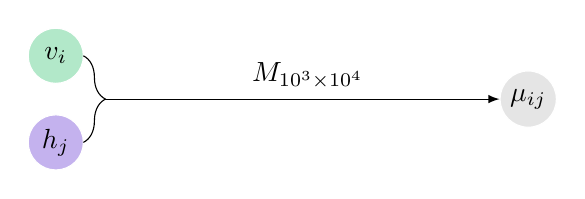
\begin{tikzpicture}
\node [minimum size=0.7cm, shape=circle,draw,inner sep=2pt, draw=white, fill=black!10] (A) at (6,-1.05) {$\mu_{ij}$};
%\node (N) at (7.5,-1.05) {$(2)$};
\node [minimum size=0.7cm, shape=circle,draw,inner sep=2pt, draw=white, fill=blue!30!green!30] (B) at (0,-0.5) {$v_i$};
\node [minimum size=0.7cm, shape=circle,draw,inner sep=2pt, draw=white, fill=purple!30!blue!30] (C) at (0,-1.6) {$h_j$};
\node (D) at (3.2,-0.75) {$M_{10^3 \times 10^4}$};
\draw[decorate, decoration={brace, mirror, amplitude=8pt}] (0.35,-1.6) -- coordinate [right=8pt] (B) (0.35,-0.5) node {};
\draw[-latex] (B) -- (A);
\end{tikzpicture}
\hspace{25pt}
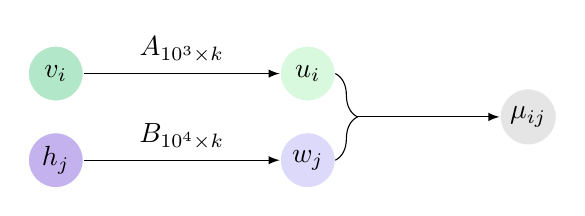
\begin{tikzpicture}
\node [minimum size=0.7cm, shape=circle,draw,inner sep=2pt, draw=white, fill=black!10] (A) at (6,-1.05) {$\mu_{ij}$};
%\node (N) at (7.5,-1.05) {$(3)$};
\node [minimum size=0.7cm, shape=circle,draw,inner sep=2pt, draw=white, fill=blue!30!green!30] (B) at (0,-0.5) {$v_i$};
\node [minimum size=0.7cm, shape=circle,draw,inner sep=2pt, draw=white, fill=purple!30!blue!30] (C) at (0,-1.6) {$h_j$};
\node [minimum size=0.7cm, shape=circle,draw,inner sep=2pt, draw=white, fill=blue!15!green!15] (E) at (3.2,-0.5) {$u_i$};
\node [minimum size=0.7cm, shape=circle,draw,inner sep=2pt, draw=white, fill=purple!15!blue!15] (F) at (3.2,-1.6) {$w_j$};
\draw[-latex] (B) -- (E);
\draw[-latex] (C) -- (F);
\node (G) at (1.6,-0.2) {$A_{10^3 \times k}$};
\node (G) at (1.6,-1.3) {$B_{10^4 \times k}$};
\draw[decorate, decoration={brace, mirror, amplitude=8pt}] (3.55,-1.6) -- coordinate [right=8pt] (E) (3.55,-0.5) node {};
\draw[-latex] (E) -- (A);
\end{tikzpicture}
\end{center}
\vspace{8pt}
\begin{center}
    \begin{tabular}{ c c c c } 
        \hline
        Solve for & Predictors & Size & Memory \\ 
        \hline
        M & $H \otimes V$ & $5.8e4 \times 1e7$ & 4.7 TB \\ 
        A & $HB \otimes V$ & $5.8e4 \times 3e3$ & 1.4 GB \\ 
        B & $H \otimes VA$ & $5.8e4 \times 3e4$ & 14 GB \\ 
        \hline
    \end{tabular}
\end{center}
\vspace{4pt}

\section{Implementation and tuning}\label{implementation-and-tuning}

The dataset was first trimmed down to a more manageable subset of 60
phage proteins and 112 host proteins by performing a first round of
lasso with only phage proteins as predictors, then another round of
lasso with only host proteins as predictors. To avoid reimplementing
regularized logistic regression, the \emph{glmnet} package in R was
used. In this smaller problem, the summary table of expected memory
usage is as follows:
\begin{center}
    \begin{tabular}{ c c c c } 
        \hline
        Solve for & Predictors & Size & Memory \\ 
        \hline
        M & $H \otimes V$ & $5.8e4 \times 6893$ & 3.2 GB \\ 
        A & $HB \otimes V$ & $5.8e4 \times 183$ & 85 MB \\ 
        B & $H \otimes VA$ & $5.8e4 \times 336$ & 156 MB \\ 
        \hline
    \end{tabular}
\end{center}
\vspace{2pt}

\subsection{Initialization}\label{initialization}

On a subset of 60 phage and 112 host proteins, M can be computed
directly. A smart way to initialize the matrices A and B would then be
to take the singular value decomposition of M. This initialization was
used as a first step in implementing alternating minimization, because
starting with values that should be much closer to optimal than random
would eliminate initialization as a possible source of failure in
implementation.

Because the goal is to use alternating minimization as a means for
working with the entire dataset, which we currently cannot do because of
memory constraints, ideally, we would like to not need to directly solve
for M. The question is then, would random initialization perform just as
well? It turns out that random initialization converges at the same rate
as SVD initialization (Figure \ref{fig:figPred}, and reaches the similar
likelihoods. This bodes well for generalizing the method to the full
dataset.
\begin{figure}[tb!]

{\centering \includegraphics[width=0.8\linewidth]{figurespred/figPred} 

}

\caption{\label{fig:figPred}Initializing A and B randomly performs comparably to initializing with the SVD of M, indicating that random initialization could still be a reasonable strategy when working with the entire dataset.}\label{fig:figPred}
\end{figure}
\subsection{Scaling A and B}\label{scaling-a-and-b}

Because \(VAB'H'\) is the inner product of \(A'V'\) and \(B'H'\), if
each predictor variable in \(V\) and \(H\) are centered and \(A\) and
\(B\) are scaled appropriately, \(A\) and \(B\) effectively project the
phage and the host, respectively, into a k dimensional space, where the
angle between phage and host that interact are low (or the correlation
is high). Therefore, if \(k\) is constrained to 2 or 3, \(A'V'\) and
\(B'H'\) can also be used for dimensionality reduction and visualization
purposes.

This geometric interpretation is somewhat thrown off by the included
intercept variables in \(V\) and \(H\), which centering would render
ineffectual. However, empirically, for solutions of \(A\) and \(B\)
which are orthogonalized after each iteration, the first dimension
always represents the intercept term. With the offset removed from the
remaining dimensions, the geometric interpretation is again recovered.
(Figure \ref{fig:figGeom})

In a sense then, this is similar to canonical correlation analysis
{[}107{]}, in which a rotation matrix is chosen for a multivariate set
of predictor variables and another rotation matrix is chosen for a
multivariate set of response variables in order to maximize the
correlation, or minimize the angle, between corresponding rows of
predictors and their responses in the first k dimensions. To make this
more concrete, a commonly used real-world example is relating
multivariate genomic data (each patient has many genomic variation, or
colloquially, mutation) to multivariate health metrics (each patient is
also associated with records of height, bmi, disease status, etc.). The
difference is that there isn't a one-to-one relationship between hosts
and phage. It's possible for a host to be susceptible to many phage, and
it's possible for a phage to be able to infect many hosts.
\begin{figure}[tb!]

{\centering \includegraphics[width=0.8\linewidth]{figurespred/figGeom} 

}

\caption{\label{fig:figGeom}When the rank of the coefficient matrices is set to 3, A and B project the phage and host genomes into a 3D space. The first dimension empirically always corresponds to the intercept. Proximity of phage and hosts in the second and third dimensions roughly corresponds to the success of infection. In this figure, the colorscheme is the same as that from before, and to emphasize the difference in organism type, phage are plotted as triangles while hosts are plotted as circles.}\label{fig:figGeom}
\end{figure}
\section{Performance engineering
results}\label{performance-engineering-results}

All analyses in this paper were performed using the R programming
language {[}108{]}. In order to assess whether these
back-of-the-envelope memory calculations hold, we profiled the code
using \emph{Rprof()}, a sampling profiler, \emph{Rprofmem()}, which
records memory usage each time memory is allocated, and \emph{gc()},
which reports memory usage whenever it is called.

\subsection{Memory}\label{memory}

Snapshots at each step of the algorithm taken using \emph{gc()} shows
that memory usage increases every time the predictors for B are
calculated, and memory usage drops when predictors for A are calculated,
as they overwrite those for B. The change in memory usage corresponds
quite well with the calculated 70 MB difference in the sizes of A and B.

Storing the values of A and B at each iteration takes up a negligible
amount of memory, as the matrices are only approximately 1.5 and 2.6 KB
respectively. For the full dataset, they would be 24 KB and 240 KB, but
still trivial, especially compared to the size of the predictor
matrices.

To address the concern that memory usage may fluctuate between the
intentionally sampled timepoints, more detailed sampling was conducted
using \emph{Rprof()} and \emph{Rprofmem()}. Results from
\emph{Rprofmem()} show that three successive memory allocation events of
the same size are made when the predictor matrices are calculated,
hinting that they may be duplicated during parameter fitting. And
indeed, \emph{Rprof()} shows that the maximum amount of memory used at
any time is three times the size of the largest matrix (the predictor
matrix for B). While this factor of three duplication still allows us to
fit to the entire dataset using \(k<=3\), additional optimization of
memory usage through implementing stochastic gradient descent will be
required.
\begin{figure}[tb!]

{\centering \includegraphics[width=0.8\linewidth]{figurespred/figMemoryPointStore} 

}

\caption{\label{fig:figMemoryPointStore}Blue points highlight operations performed in order to solve for A, the matrix of phage protein coefficients, and tan points highlight operations performed in order to solve for B, the matrix of host protein coefficients. Alternating grey and white backgrounds demarcate successive iterations. Snapshots at each step of the algorithm shows that memory usage increases every time the predictors for B are calculated, and memory usage drops when predictors for A are calculated, as they overwrite those for B.}\label{fig:figMemoryPointStore}
\end{figure}
\subsection{Runtime}\label{runtime}

The amount of wall time used to solve for the entire matrix is roughly
equivalent to performing 6 or 7 iterations of alternating minimization.
At this point, the log likelihood is within a threshold of 0.001 times
the magnitude of the log likelihood from the last iteration. This is a
reasonable stopping point, and so for this trimmed dataset at a rank set
to 3, there is very little time trade-off for the increased efficiency
of memory usage. The trade-off, however, comes in the modeling.
\begin{figure}[tb!]

{\centering \includegraphics[width=0.8\linewidth]{figurespred/figTimePointStore} 

}

\caption{\label{fig:figTimePointStore}Because parameter optimization involves searching in a high-dimensional space, the steps of solving for A and B are inevitably the rate-limiting steps of the method. Directly fitting the matrix M takes 1352 seconds (22 minutes) on the same machine.}\label{fig:figTimePointStore}
\end{figure}
\subsection{Correspondence with the original
model}\label{correspondence-with-the-original-model}

It is comforting to see in figure \ref{fig:figllcorsvd} that the
correlation between parameters from fitting \(M\) directly and
parameters from computing \(AB'\) after alternating minimization climbs
with each iteration of the algorithm. However, the correlation only
reaches 0.38 (when excluding the intercept term), and the log likelihood
only reaches -2100 (whereas the log likelihood solving for M directly is
-1460). This isn't too surprising, given that for this analysis, the
rank has been set to 3.

Inspection of the eigenvalues from singular value decomposition in the
third panel of figure \ref{fig:figllcorsvd} can give us a hint as to
what a more realistic value of k should be. However, it is still
difficult to interpolate to the full dataset, as the procedure for
picking predictors to form the smaller dataset selects variables with
high explanatory power. In general, even in the problem of matrix
completion, it is not well understood how k should be set. This is a
question for future exploration.
\begin{figure}[tb!]

{\centering \includegraphics[width=1\linewidth]{figurespred/figllcorsvd} 

}

\caption{\label{fig:figllcorsvd}In the first two plots here, the log likelihood and correlation with M (excluding the intercept term, the intercept term is so low in magnitude and so consistent with fitting that including it bumps up the correlation to around 0.97) are plotted for each iteration. Initial values are left off from these plots, since, because the parameters are randomly initialized, the log likelihood starts at -Inf and the correlation starts close to 0. The eigenvalues from singular value decomposition of the coefficient matrix M when solving for M directly is shown in the third plot. The first dimension is left off, since it is a value large in magnitude, corresponding to the intercept.}\label{fig:figllcorsvd}
\end{figure}
\section{Additional directions for
exploration}\label{additional-directions-for-exploration}

This implementation of alternating minimization is only the first step
in the analysis of the Nahant Collection. Matrices in R have been
traditionally constrained to having less than \(2^{31}\) entries, and
for \(k>3\), unfortunately, \(58,000 \times 10,000 * k\) surpasses
\(2^31\). While the most recent release of R allows larger matrices,
many packages, including \emph{glmnet}, do not yet support this new data
structure. So in order to work with \(k\) larger than 3, we will need to
reimplement elastic net regression.

Additionally, because living organisms can intuitively be placed on a
tree, there naturally exists correlation among the bacteria and among
the phage. This means that the data is not independently and identically
distributed. Our next step is to account for this in order to, as much
as possible, avoid identifying spurious associations.

Furthermore, because \(p>>n\) the interpretability of parameter
estimates is often given up as a hopeless task. Many traditional
statisticians will steer away from these types of problems, and in the
``machine learning'' community, the focus is instead on predictive
accuracy. A philosophical question also exists in whether it may, in
fact, be ill-advised to seek interpretation or draw any type of
inferences whatsoever from this type of data. To address this concern,
we turn to Tukey, ``Danger only comes from mathematical optimizing when
the results are taken too seriously\ldots{} It is understood that such
optimum problems are unrealistically oversimplified, that they offer
\emph{guidance}, not the \emph{answer}'' We cannot claim that our
analysis will be able to root the precise cause of each infection event.
Rather, we would simply like to generate testable hypotheses concerning
infection mechanisms.

Key to interpretation of parameter estimates is quantifying their
uncertainty, and alternating minimization adds another layer of
complication in that the original parameters of interest are now vector
products of parameters we have solved for. However, taking a bayesian
approach may help with this problem, as deriving the probability
distribution of sums and products of other quantities with known
distributions is straightforward.

\chapter{Reasoning Through Games of Chance - Statistics for
Play}\label{reasoning-through-games-of-chance---statistics-for-play}

\singlespace
Joy Y. Yang\(^1\), Joseph Elsherbini\(^2\) \newline 

\noindent \(^1\)Computational and Systems Biology Program, Massachusetts
Institute of Technology, Cambridge, Massachusetts 02139, USA

\noindent \(^3\)Microbiology Graduate Program, Massachusetts Institute
of Technology, Cambridge, Massachusetts 02139, USA

\noindent J.Y. and J.E. designed the curriculum, taught the class, and
wrote this paper. \newline

\noindent This paper was originally accepted as a contributed paper to
ICOTS10; however, due to scheduling conflicts, neither author was able
to attend and present the paper.

\doublespace
\newpage

\section{Abstract}\label{abstract-3}

We present a case study of a best attempt at creating a fun and
approachable after school statistics curriculum for grades 7-12. Our
goal was to use interactive games to provide intuition into a broad
range of problems that can be tackled with statistical thinking, as
opposed to teaching a comprehensive statistics immersion program. For
example, we reviewed distributions by carrying out Fisher's
hypergeometric taste testing experiment; introduced game theory by
holding an iterated prisoners' dilemma tournament; and ``because danger
only comes from mathematical optimizing when the results are taken too
seriously'' (Tukey {[}109{]}), ended with correlation/causation critical
thinking puzzles. Additionally, we will discuss lessons learned from
attempting to synthesize many activity based learning and context-driven
statistical education tools that have arisen from conferences such as
ICOTS.

\section{Introduction}\label{introduction-3}

We've designed a six-session summer weekend curriculum consisting of
games, in the spirit of Box's paper helicopter experiments, {[}110{]}
that seeks to elicit the context of need under which various statistical
analyses were developed/are employed. In this paper, we will first
introduce the setting under which we've taught this class, then comment
on our experience of designing and running the class, and finally
discuss the arguments for teaching in this manner by summarizing the
viewpoints of seasoned statisticians who have thought deeply about
activity-based and context-driven statistical education. Our materials
for this class are available at \url{http://mit.edu/reasoningchance/}

\section{MIT HSSP}\label{mit-hssp}

MIT Summer HSSP (this acronym has no expanded meaning) is a 6-week
7-12th grade program that runs on Sunday afternoons. Students can
register for multiple classes, and MIT-affiliates (undergraduates,
graduate students, or alumni) can apply to teach a class of any topic.
The MIT Educational Studies Program (ESP) handles the logistics of doing
outreach at local schools, recruiting teachers, selecting classes, and
reserving classrooms. During 2017, around 1500 students enrolled, and 44
different classes were offered over a wide range of topics: swing
dancing, complex analysis, adulting 101; etc. MIT ESP encourages
students to leave the classroom if they find that they are not enjoying
the material.

Under this program, we piloted a probability/statistics teaser series
called ``Reasoning through games of chance.'' The afterschool program
format meant that our lesson plans could not be a regimented,
comprehensive overview of statistics. Instead, we indulged in
prioritizing fun and intuition, with the aim of encouraging students to
think about where, in their lives, chance and data play a role, and how
they can use probability and statistics to explore their environment.

\section{Class Setup}\label{class-setup}

While we did not require programming as a prerequisite and did not plan
to teach students how to code, we wanted students to realize that
statistics is deeply intertwined with computing, as eloquently expressed
by {[}111{]}. To this end, we requested the use of laptops and were
given access to 12 chromebooks. The class size was then limited to 24
students so that each group of 2 students could work with one
chromebook. Each chromebook was associated with a google classroom
account to facilitate distribution of activities and interaction among
groups.

We also prepared short code snippets on Rfiddle
(\url{http://www.r-fiddle.org/}) to demonstrate basic functions and
simulations. Because saving fiddles creates urls with different version
numbers, we could update the fiddles live and ask students to follow
along by navigating to newer versions. Students were also encouraged to
continue playing with the code on their own time.

The students were from a wide range of different schools and grades.
This sounds challenging; however, we believe it worked to our advantage.
Each class was almost entirely activity based. So while in theory, our
goal was to teach using guiding questions, in reality, the students
taught each other.
\begin{figure}[tb!]

{\centering \includegraphics[width=0.9\linewidth]{figuresteaching/studentDem} 

}

\caption{\label{fig:studentDem}This map omits two students, one from Maine, another from Illinois.}\label{fig:studentDem}
\end{figure}
In general, we tried to encourage as much discussion as possible and
aimed to maintain an atmosphere of organized chaos. And while the
precise class structure varied from week to week, the scaffolding we
used for planning was somewhat consistent: we started with an
ice-breaker, followed with drill exercises, and ended with an
experiment, or ``game.''

To provide an example, we will use class 2: distributions and hypothesis
testing. The learning goal was to expose students to the concept of a
``null model,'' and encourage them to consider what a null outcome
should look like.

The icebreaker (\textasciitilde{}10-20 min) was often only tangentially
related to the main topic. Because there are many ways of approaching
the same problem, and problems can often be reduced to each other, these
tangents allowed us to point out subtle connections among topics. Our
icebreaker in class 2 was a classification problem. Pairs of students
were given 12 labeled images that fell into two categories, for example,
chessboards from either early in the game or late in a game. Students
were then asked to come up with rules that categorized their images. For
instance, a rule might be ``the image is from (early/late) in the game
if the number of pawns on the board is (less than/equal-to/greater than)
c.'' After the students designed a set of rules, we then gave them 4
additional images to test how well their rules did.

For the drill exercises (\textasciitilde{}20-40 min), we typically asked
students to number off into groups of four, then work out the answers
together on board space marked for each group. Because the icebreakers
were usually very open ended, and the games focused on having fun, these
more structured exercises were intended to hone in on the relevant
concepts of the week. Using boards helped promote interaction within the
groups and allowed us, as the teachers, to easily identify and
brainstorm with groups that looked stuck. The drill exercises in class 2
aimed to reinforce concept of distributions. There were two parts: In
part one, students answered various questions about heights of
Lilliputians by reading a histogram, and were then asked how likely it
was Gulliver was a Lilliputian. In part two, students were given
sequences of coin-flips and guided through deducing the geometric
distribution by calculating probabilities for runs of heads and tails.
They then used this information to determine which sequences were from
real coin flips and which were faked by the instructors. Half of the
groups worked on part one and the other half on part two. After everyone
had finished, the groups swapped boards to discussed/corrected another
group's work.

Finally, the goals for the games (\textasciitilde{}30-40 min) were to
demonstrate that statistical thinking is fun and to provide an example
of how students can apply probability and statistics in their own lives.
In class 2, the game was a taste testing experiment. We had three
different tests: skittles vs.~m\&ms, coke vs.~pepsi, and different
colors of vegetable chips. Students worked in groups of three to
administer the tests and record the results in a linked spreadsheet. We
then briefly talked about the hypergeometric distribution as a null and
showed the students the distribution of their cell counts compared to
the null. Students were then asked to explain what the visualizations
meant and whether we had evidence that people could discriminate between
the different foods.

\section{Reflection and Outlook}\label{reflection-and-outlook}

Statistical thinking is a necessary companion of the scientific process;
or if we dare to go as far as Stigler, statistics is ``a unified logic
of empirical science.'' A corollary to this, as stated poignantly by
Rebecca Nugent in her JSM 2017 talk {[}112{]}, is that ``statistics does
not belong to statisticians, statistical questions are present in every
field, from physics, to chemistry, to history.'' So in an attempt to
attract as diverse a group of students as possible, we required no
pre-requisites, marked the difficulty for our class to be 1 (on the
scale of 1-4, 1 being the lowest), and welcomed students from the entire
range of 7-12 grade. Still, there's quite a bit of selection bias
present in a group of students who come to MIT on weekends in the
summer. When asked what their favorite subject were, most of our
students said math, and only one student said English. Our students were
incredibly supportive. They were eager to have fun and quick to come up
with entirely unexpected responses.
\begin{figure}[tb!]

{\centering \includegraphics[width=1\linewidth]{figuresteaching/sheep} 

}

\caption{\label{fig:sheep}When asked to summarize the sheep in their herd, one group responded with pictorial summaries.}\label{fig:sheep}
\end{figure}
We designed the activities to focus on intuition, and did not attempt to
be mathematically rigorous. We did attempt to teach the Bayes class
using probability notation, and our students became uncharacteristically
frustrated. We had not built up the intuition before introducing the
symbols, and so the symbols carried no meaning. To the final question of
a worksheet (``what are some ways that you can increase the accuracy of
the test?''), one student responded, ``math, solve your own problems.''
We found this humorous but also alarming. This student had come in with
math as her favorite subject, and we had a responsibility for
encouraging her mathematical curiosity, or at the very least, for not
discouraging her. So after class we sent a out new explanation based on
intuition. We also reworked the lesson plan to no longer use probability
notation. This new lesson plan was tested on November 18-19, and seemed
to be received with greater success. However, the class sizes were also
smaller, so there may have been some amount of confounding.

Focusing on intuition has a twofold advantage: as {[}113{]} pointed out,
in democratizing statistics we should ``avoid the `professional's
fallacy' of imagining that our first courses are a step in the training
of statisticians.'' For students who do not choose to continue on with
statistics, it is the big picture ideas, and not the fine-grained
details that will leave a lasting impression. And for students who do
decide to pursue statistics, again quoting {[}114{]}, ``most of our
students would better master theory after some acquaintance with
practice.''

Gudmund Iversen explains from his experience: ``Those students who have
had my Statistical Thinking course early (freshmen, sophomores) are
having a ball with mathematical statistics as juniors or seniors. Others
struggle more because they get bogged down by probability theory and
mathematical niceties like moment generating functions, and they have a
harder time seeing what statistics is all about. This points to a need
to hear statistics twice before it makes sense, and we cannot lose the
connection to real data.'' {[}115{]} Our hope was that by placing
emphasis on simply having fun, we could plant a seed to mark a spot that
students may conceivably want to revisit, sooner rather than later.

One advantage we had during HSSP is that we had a returning group of
students over the course of six weeks, so we were able to refer back to
examples from previous classes. However, we realize that running
examples can create barriers to entry, and many after-school programs
may not have the luxury of continuity. So in order to increase the
accessibility and versatility of this set of lesson plans, we've also
adapted three of the classes from this series for SPLASH, another MIT
ESP program with a one-weekend-only format, held, this year, November
18-19.

While we do not have enough space here to discuss SPLASH in detail,
interestingly, we had a very different audience. Only about 10\% of our
students said Math was their favorite subject, and one student made a
seemingly outlandish comment about hating the coordinate system when he
first learned about it. When asked to elaborate, he said, ``In school
they have you draw this Cartesian grid, and then plot things like lines
on it, but it seemed pretty pointless. Then, I realized that you can
actually graph food or baseball statistics, and I became a lot more
interested. I'm not really bad at math, but most of the times it just
seems really pointless and boring to me, because they don't tell you
what you can use it for.'' Behind each statistical method, there are
many fascinating stories about how it is used. Playfully invoking these
contexts makes statistics relatable {[}116--118{]}, and we are excited
about the prospect of using this thought process to design additional
afterschool lesson plans that are accessible at the jr. high/high school
level.

\section{Acknowledgements}\label{acknowledgements-2}

We'd like to thank to Max Shen and Hayley Gadol for co-teaching. We also
owe so many thanks to Luke Miratrix for activity ideas and feedback on
the agendas for most of our lesson plans as well as this paper. Our
curriculum benefitted greatly from activities developed previously by
others. {[}119--121{]} An interest in context-based education came from
many dinner-table conversations among friends (Leanne Fan, Charlie Shi,
Matt Nickell, and Kelly Vitzhum) that evolved into writing an education
grant. While we did not receive the grant, this concept has become a
mild obsession for each of us in our respective fields. And finally,
we'd like Libusha Kelly for her thoughtful comments on this paper.

\backmatter

\chapter*{References}\label{references}
\addcontentsline{toc}{chapter}{References}

\markboth{References}{References}

\noindent

\setlength{\parindent}{-0.20in} \setlength{\leftskip}{0.20in}
\setlength{\parskip}{8pt} \singlespacing

\hypertarget{refs}{}
\hypertarget{ref-Brillinger2002}{}
1. Brillinger DR (2002) John W. Tukey: his life and professional
contributions. The Annals of Statistics 30:1535--1575. doi:
\href{https://doi.org/10.1214/aos/1043351246}{10.1214/aos/1043351246}

\hypertarget{ref-Bergh1989}{}
2. Bergh O, Børsheim KY, Bratbak G, Heldal M (1989) High abundance of
viruses found in aquatic environments. Nature 340:467--8. doi:
\href{https://doi.org/10.1038/340467a0}{10.1038/340467a0}

\hypertarget{ref-nasa}{}
3. (2015) The North Sea Abloom : Image of the Day.

\hypertarget{ref-Wilson2002}{}
4. Wilson WH, Tarran GA, Schroeder D, et al. (2002) Isolation of viruses
responsible for the demise of an Emiliania huxleyi bloom in the English
Channel.

\hypertarget{ref-Schroeder2003}{}
5. Schroeder DC, Oke J, Hall M, et al. (2003) Virus succession observed
during an Emiliania huxleyi bloom. Applied and environmental
microbiology 69:2484--90.

\hypertarget{ref-Hyman2010}{}
6. Hyman P, Abedon ST (2010) Chapter 7 -- Bacteriophage Host Range and
Bacterial Resistance. In: Advances in applied microbiology. pp 217--248

\hypertarget{ref-Fuhrman1999}{}
7. Fuhrman JA (1999) Marine viruses and their biogeochemical and
ecological effects. Nature 399:541--8. doi:
\href{https://doi.org/10.1038/21119}{10.1038/21119}

\hypertarget{ref-Wilhelm2002}{}
8. Wilhelm S, Brigden S, Suttle C (2002) A Dilution Technique For The
Direct Measurement Of Viral Production: A Comparison In Stratified And
Tidally Mixed Coastal Waters. Microbial Ecology 43:168--173. doi:
\href{https://doi.org/10.1007/s00248-001-1021-9}{10.1007/s00248-001-1021-9}

\hypertarget{ref-Hendrix2003}{}
9. Hendrix RW (2003) Bacteriophage genomics. Current Opinion in
Microbiology 6:506--511. doi:
\href{https://doi.org/10.1016/J.MIB.2003.09.004}{10.1016/J.MIB.2003.09.004}

\hypertarget{ref-Hendrix1999}{}
10. Hendrix RW, Smith MC, Burns RN, et al. (1999) Evolutionary
relationships among diverse bacteriophages and prophages: all the
world's a phage. Proceedings of the National Academy of Sciences of the
United States of America 96:2192--7.

\hypertarget{ref-Gonzalez2015}{}
11. González V, Lozano L, Bustos P, Santamaría RI (2015) Genomic Tools
for the Study of Azospirillum and Other Plant Growth-Promoting
Rhizobacteria. In: Handbook for azospirillum. Springer International
Publishing, Cham, pp 83--97

\hypertarget{ref-Griffiths2000}{}
12. Griffiths AJF (2000) An introduction to genetic analysis. 860.

\hypertarget{ref-Salmond2015}{}
13. Salmond GPC, Fineran PC (2015) A century of the phage: past, present
and future. Nature Reviews Microbiology 13:777--786. doi:
\href{https://doi.org/10.1038/nrmicro3564}{10.1038/nrmicro3564}

\hypertarget{ref-Maloy}{}
14. Maloy S Insights from Phage.

\hypertarget{ref-Luria1943}{}
15. Luria SE, Delbrück M (1943) Mutations of Bacteria from Virus
Sensitivity to Virus Resistance. Genetics 28:

\hypertarget{ref-HERSHEY1952}{}
16. Hershey AD, Chase M (1952) Independent functions of viral protein
and nucleic acid in growth of bacteriophage. The Journal of general
physiology 36:39--56.

\hypertarget{ref-Benzer}{}
17. Benzer S Fine Structure of a Genetic Region in Bacteriophage.
41:344--354. doi: \href{https://doi.org/10.2307/89013}{10.2307/89013}

\hypertarget{ref-Benzera}{}
18. Benzer S On the Topology of the Genetic Fine Structure.
45:1607--1620. doi: \href{https://doi.org/10.2307/90127}{10.2307/90127}

\hypertarget{ref-CRICK1961}{}
19. Crick FHC, Barnett L, Brenner S, Watts-Tobin RJ (1961) General
Nature of the Genetic Code for Proteins. Nature 192:1227--1232. doi:
\href{https://doi.org/10.1038/1921227a0}{10.1038/1921227a0}

\hypertarget{ref-Summers}{}
20. Summers WC How Bacteriophage Came to Be Used by the Phage Group.
26:255--267. doi:
\href{https://doi.org/10.2307/4331263}{10.2307/4331263}

\hypertarget{ref-Ellis1939}{}
21. Ellis EL, Delbrück M (1939) The Growth of Bacteriophage. The Journal
of general physiology 22:365--84.

\hypertarget{ref-Boland1984}{}
22. Boland PJ (1984) A Biographical Glimpse of William Sealy Gosset. The
American Statistician 38:179--183. doi:
\href{https://doi.org/10.1080/00031305.1984.10483195}{10.1080/00031305.1984.10483195}

\hypertarget{ref-Clarke1946}{}
23. Clarke RD (1946) An application of the Poisson distribution. Journal
of the Institute of Actuaries 72:481--481. doi:
\href{https://doi.org/10.1017/S0020268100035435}{10.1017/S0020268100035435}

\hypertarget{ref-sequencingcosts}{}
24. DNA Sequencing Costs: Data - National Human Genome Research
Institute (NHGRI).

\hypertarget{ref-Pesant2015}{}
25. Pesant S, Not F, Picheral M, et al. (2015) Open science resources
for the discovery and analysis of Tara Oceans data. Scientific Data
2:150023. doi:
\href{https://doi.org/10.1038/sdata.2015.23}{10.1038/sdata.2015.23}

\hypertarget{ref-Brum2015}{}
26. Brum JR, Ignacio-Espinoza JC, Roux S, et al. (2015) Patterns and
ecological drivers of ocean viral communities. Science (New York, NY)
348:1261498. doi:
\href{https://doi.org/10.1126/science.1261498}{10.1126/science.1261498}

\hypertarget{ref-Pope2015}{}
27. Pope WH, Bowman CA, Russell DA, et al. (2015) Whole genome
comparison of a large collection of mycobacteriophages reveals a
continuum of phage genetic diversity. eLife. doi:
\href{https://doi.org/10.7554/eLife.06416}{10.7554/eLife.06416}

\hypertarget{ref-Kauffman2014}{}
28. Kauffman AKM (2014) Demographics of lytic viral infection of coastal
ocean vibrio.

\hypertarget{ref-Kauffman2018}{}
29. Kauffman KM, Hussain FA, Yang J, et al. (2018) A major lineage of
non-tailed dsDNA viruses as unrecognized killers of marine bacteria.
Nature 554:118--122. doi:
\href{https://doi.org/10.1038/nature25474}{10.1038/nature25474}

\hypertarget{ref-Kauffman2018a}{}
30. Kauffman KM, Brown JM, Sharma RS, et al. (2018) Viruses of the
Nahant Collection, characterization of 251 marine Vibrionaceae viruses.
Scientific Data 5:180114. doi:
\href{https://doi.org/10.1038/sdata.2018.114}{10.1038/sdata.2018.114}

\hypertarget{ref-Hunt2008}{}
31. Hunt DE, David LA, Gevers D, et al. (2008) Resource partitioning and
sympatric differentiation among closely related bacterioplankton.
Science (New York, NY) 320:1081--5. doi:
\href{https://doi.org/10.1126/science.1157890}{10.1126/science.1157890}

\hypertarget{ref-Preheim2011}{}
32. Preheim SP, Boucher Y, Wildschutte H, et al. (2011) Metapopulation
structure of Vibrionaceae among coastal marine invertebrates.
Environmental Microbiology 13:265--275. doi:
\href{https://doi.org/10.1111/j.1462-2920.2010.02328.x}{10.1111/j.1462-2920.2010.02328.x}

\hypertarget{ref-Stone2011}{}
33. Stone GN, Nee S, Felsenstein J (2011) Controlling for
non-independence in comparative analysis of patterns across populations
within species. Philosophical transactions of the Royal Society of
London Series B, Biological sciences 366:1410--24. doi:
\href{https://doi.org/10.1098/rstb.2010.0311}{10.1098/rstb.2010.0311}

\hypertarget{ref-Felsenstein2008}{}
34. Felsenstein J (2008) Comparative methods with sampling error and
within-species variation: contrasts revisited and revised. The American
naturalist 171:713--25. doi:
\href{https://doi.org/10.1086/587525}{10.1086/587525}

\hypertarget{ref-Cheverud1985}{}
35. Cheverud J (1985) The quantitative assessment of phylogenetic
constraints in comparative analyses: sexual dimorphism in body weight
among primates.

\hypertarget{ref-Price2006}{}
36. Price AL, Patterson NJ, Plenge RM, et al. (2006) Principal
components analysis corrects for stratification in genome-wide
association studies. Nature Genetics 38:904--909. doi:
\href{https://doi.org/10.1038/ng1847}{10.1038/ng1847}

\hypertarget{ref-PAGEL1997}{}
37. Pagel M (1997) Inferring evolutionary processes from phylogenies.
Zoologica Scripta 26:331--348. doi:
\href{https://doi.org/10.1111/j.1463-6409.1997.tb00423.x}{10.1111/j.1463-6409.1997.tb00423.x}

\hypertarget{ref-Hadfield}{}
38. Hadfield J MCMCglmm Course Notes.

\hypertarget{ref-Hadfield2010a}{}
39. Hadfield JD, Nakagawa S (2010) General quantitative genetic methods
for comparative biology: phylogenies, taxonomies and multi-trait models
for continuous and categorical characters. Journal of evolutionary
biology 23:494--508. doi:
\href{https://doi.org/10.1111/j.1420-9101.2009.01915.x}{10.1111/j.1420-9101.2009.01915.x}

\hypertarget{ref-Hadfield2010}{}
40. Hadfield JD (2010) MCMC Methods for Multi-Response Generalized
Linear Mixed Models: The MCMCglmm R Package.

\hypertarget{ref-Brillinger}{}
41. Brillinger DR Data Analysis, Exploratory. International encyclopedia
of political science. doi:
\href{https://doi.org/10.4135/9781412959636.n128}{10.4135/9781412959636.n128}

\hypertarget{ref-Tukey1977}{}
42. Tukey JW(W (1977) Exploratory data analysis. 688.

\hypertarget{ref-Cowe1991}{}
43. Cowe E, Sharp PM (1991) Molecular evolution of bacteriophages:
Discrete patterns of codon usage in T4 genes are related to the time of
gene expression. Journal of Molecular Evolution 33:13--22. doi:
\href{https://doi.org/10.1007/BF02100191}{10.1007/BF02100191}

\hypertarget{ref-Scola}{}
44. La Scola B, Audic S, Robert C, et al. (2003) A giant virus in
amoebae. sciencesciencemagorg 299:2033.

\hypertarget{ref-Raoult2004}{}
45. Raoult D, Audic S, Robert C, et al. (2004) The 1.2-megabase genome
sequence of Mimivirus. Science (New York, NY) 306:1344--50. doi:
\href{https://doi.org/10.1126/science.1101485}{10.1126/science.1101485}

\hypertarget{ref-Abergel2015}{}
46. Abergel C, Legendre M, Claverie J-M (2015) The rapidly expanding
universe of giant viruses: Mimivirus, Pandoravirus, Pithovirus and
Mollivirus. FEMS Microbiology Reviews 39:779--796. doi:
\href{https://doi.org/10.1093/femsre/fuv037}{10.1093/femsre/fuv037}

\hypertarget{ref-Schulz2017}{}
47. Schulz F, Yutin N, Ivanova NN, et al. (2017) Giant viruses with an
expanded complement of translation system components. Science (New York,
NY) 356:82--85. doi:
\href{https://doi.org/10.1126/science.aal4657}{10.1126/science.aal4657}

\hypertarget{ref-Hatfull2008}{}
48. Hatfull GF (2008) Bacteriophage genomics. Current opinion in
microbiology 11:447--53. doi:
\href{https://doi.org/10.1016/j.mib.2008.09.004}{10.1016/j.mib.2008.09.004}

\hypertarget{ref-Daniel1968}{}
49. Daniel V, Sarid S, Littauer U (1968) Amino acid acceptor activity of
bacteriophage T4 transfer RNA. FEBS Letters 2:39--41. doi:
\href{https://doi.org/10.1016/0014-5793(68)80095-X}{10.1016/0014-5793(68)80095-X}

\hypertarget{ref-Weiss1968}{}
50. Weiss SB, Hsu WT, Foft JW, Scherberg NH (1968) Transfer RNA coded by
the T4 bacteriophage genome. Proceedings of the National Academy of
Sciences of the United States of America 61:114--21.

\hypertarget{ref-Scherberg1972}{}
51. Scherberg NH, Weiss SB (1972) T4 transfer RNAs: codon recognition
and translational properties. Proceedings of the National Academy of
Sciences of the United States of America 69:1114--8. doi:
\href{https://doi.org/10.1073/PNAS.69.5.1114}{10.1073/PNAS.69.5.1114}

\hypertarget{ref-Wilson1973}{}
52. Wilson JH (1973) Function of the bacteriophage T4 transfer RNA's.
Journal of Molecular Biology 74:753--757. doi:
\href{https://doi.org/10.1016/0022-2836(73)90065-X}{10.1016/0022-2836(73)90065-X}

\hypertarget{ref-Matsuzaki1992}{}
53. Matsuzaki S, Tanaka S, Koga T, Kawata T (1992) A Broad-Host-Range
Vibriophage, KVP40, Isolated from Sea Water. Microbiology and Immunology
36:93--97. doi:
\href{https://doi.org/10.1111/j.1348-0421.1992.tb01645.x}{10.1111/j.1348-0421.1992.tb01645.x}

\hypertarget{ref-Miller2003}{}
54. Miller ES, Heidelberg JF, Eisen JA, et al. (2003) Complete genome
sequence of the broad-host-range vibriophage KVP40: comparative genomics
of a T4-related bacteriophage. Journal of bacteriology 185:5220--33.

\hypertarget{ref-Ikemura1981}{}
55. Ikemura T (1981) Correlation between the abundance of Escherichia
coli transfer RNAs and the occurrence of the respective codons in its
protein genes: A proposal for a synonymous codon choice that is optimal
for the E. coli translational system. Journal of Molecular Biology
151:389--409. doi:
\href{https://doi.org/10.1016/0022-2836(81)90003-6}{10.1016/0022-2836(81)90003-6}

\hypertarget{ref-Sharp2010}{}
56. Sharp PM, Emery LR, Zeng K (2010) Forces that influence the
evolution of codon bias. Philosophical transactions of the Royal Society
of London Series B, Biological sciences 365:1203--12. doi:
\href{https://doi.org/10.1098/rstb.2009.0305}{10.1098/rstb.2009.0305}

\hypertarget{ref-Grantham1980}{}
57. Grantham R, Gautier C, Gouy M, et al. (1980) Codon catalog usage and
the genome hypothesis. Nucleic acids research 8:r49--r62.

\hypertarget{ref-Botzman2011}{}
58. Botzman M, Margalit H (2011) Variation in global codon usage bias
among prokaryotic organisms is associated with their lifestyles. Genome
biology 12:R109. doi:
\href{https://doi.org/10.1186/gb-2011-12-10-r109}{10.1186/gb-2011-12-10-r109}

\hypertarget{ref-Bailly-Bechet2007}{}
59. Bailly-Bechet M, Vergassola M, Rocha E (2007) Causes for the
intriguing presence of tRNAs in phages. Genome research 17:1486--95.
doi: \href{https://doi.org/10.1101/gr.6649807}{10.1101/gr.6649807}

\hypertarget{ref-Delesalle2016}{}
60. Delesalle VA, Tanke NT, Vill AC, Krukonis GP (2016) Testing
hypotheses for the presence of tRNA genes in mycobacteriophage genomes.
Bacteriophage 6:e1219441. doi:
\href{https://doi.org/10.1080/21597081.2016.1219441}{10.1080/21597081.2016.1219441}

\hypertarget{ref-DosReis2004}{}
61. Reis M dos, Savva R, Wernisch L (2004) Solving the riddle of codon
usage preferences: a test for translational selection. Nucleic acids
research 32:5036--44. doi:
\href{https://doi.org/10.1093/nar/gkh834}{10.1093/nar/gkh834}

\hypertarget{ref-Watanabe1995}{}
62. Watanabe K, Osawa S (1995) tRNA sequences and variation in the
genetic code. In: Söll D, Rajbhandary U (eds) TRNA: Structure,
biosynthesis, and function. ASM Press, Washington, DC, pp 225--250

\hypertarget{ref-Yokoyama1995}{}
63. Yokoyama S, Nishimura S (1995) Modified nucleosides and codon
recognition. In: Söll D, RajBhandary UL (eds) TRNA: Structure,
biosynthesis, and function. ASM Press, Washington, DC, pp 207--223

\hypertarget{ref-Reiter1989}{}
64. Reiter WD, Palm P, Yeats S (1989) Transfer RNA genes frequently
serve as integration sites for prokaryotic genetic elements. Nucleic
acids research 17:1907--14.

\hypertarget{ref-Williams2002}{}
65. Williams KP (2002) Integration sites for genetic elements in
prokaryotic tRNA and tmRNA genes: sublocation preference of integrase
subfamilies. Nucleic acids research 30:866--75.

\hypertarget{ref-Johnson2015}{}
66. Johnson CM, Grossman AD (2015) Integrative and Conjugative Elements
(ICEs): What They Do and How They Work. Annual review of genetics
49:577--601. doi:
\href{https://doi.org/10.1146/annurev-genet-112414-055018}{10.1146/annurev-genet-112414-055018}

\hypertarget{ref-Marquet1995}{}
67. Marquet R, Isel C, Ehresmann C, Ehresmann B (1995) tRNAs as primer
of reverse transcriptases. Biochimie 77:113--124. doi:
\href{https://doi.org/10.1016/0300-9084(96)88114-4}{10.1016/0300-9084(96)88114-4}

\hypertarget{ref-Kleiman2002}{}
68. Kleiman L (2002) tRNALys3: The Primer tRNA for Reverse Transcription
in HIV-1. IUBMB Life (International Union of Biochemistry and Molecular
Biology: Life) 53:107--114. doi:
\href{https://doi.org/10.1080/15216540211469}{10.1080/15216540211469}

\hypertarget{ref-Hou2010}{}
69. Hou Y-M (2010) CCA addition to tRNA: implications for tRNA quality
control. IUBMB life 62:251--60. doi:
\href{https://doi.org/10.1002/iub.301}{10.1002/iub.301}

\hypertarget{ref-Korostelev2006}{}
70. Korostelev A, Trakhanov S, Laurberg M, Noller HF (2006) Crystal
Structure of a 70S Ribosome-tRNA Complex Reveals Functional Interactions
and Rearrangements. Cell 126:1065--1077. doi:
\href{https://doi.org/10.1016/j.cell.2006.08.032}{10.1016/j.cell.2006.08.032}

\hypertarget{ref-Dupasquier2008}{}
71. Dupasquier M, Kim S, Halkidis K, et al. (2008) tRNA integrity is a
prerequisite for rapid CCA addition: implication for quality control.
Journal of molecular biology 379:579--88. doi:
\href{https://doi.org/10.1016/j.jmb.2008.04.005}{10.1016/j.jmb.2008.04.005}

\hypertarget{ref-Clark2016}{}
72. Clark WC, Evans ME, Dominissini D, et al. (2016) tRNA base
methylation identification and quantification via high-throughput
sequencing. RNA 22:1771--1784. doi:
\href{https://doi.org/10.1261/rna.056531.116}{10.1261/rna.056531.116}

\hypertarget{ref-Harada1974}{}
73. Harada F, Nishimura S (1974) Purification and characterization of
AUA specific isoleucine transfer ribonucleic acid from Escherichia coli
B. Biochemistry 13:300--307. doi:
\href{https://doi.org/10.1021/bi00699a011}{10.1021/bi00699a011}

\hypertarget{ref-Lowe1997}{}
74. Lowe TM, Eddy SR (1997) tRNAscan-SE: a program for improved
detection of transfer RNA genes in genomic sequence. Nucleic acids
research 25:955--64.

\hypertarget{ref-Laslett2004}{}
75. Laslett D, Canback B (2004) ARAGORN, a program to detect tRNA genes
and tmRNA genes in nucleotide sequences. Nucleic acids research
32:11--6. doi:
\href{https://doi.org/10.1093/nar/gkh152}{10.1093/nar/gkh152}

\hypertarget{ref-Enav2012}{}
76. Enav H, Béjà O, Mandel-Gutfreund Y (2012) Cyanophage tRNAs may have
a role in cross-infectivity of oceanic Prochlorococcus and Synechococcus
hosts. The ISME journal 6:619--28. doi:
\href{https://doi.org/10.1038/ismej.2011.146}{10.1038/ismej.2011.146}

\hypertarget{ref-Davis1986}{}
77. Davis BD, Luger SM, Tai PC (1986) Role of ribosome degradation in
the death of starved Escherichia coli cells. Journal of bacteriology
166:439--45.

\hypertarget{ref-Zhong2015}{}
78. Zhong J, Xiao C, Gu W, et al. (2015) Transfer RNAs Mediate the Rapid
Adaptation of Escherichia coli to Oxidative Stress. PLOS Genetics
11:e1005302. doi:
\href{https://doi.org/10.1371/journal.pgen.1005302}{10.1371/journal.pgen.1005302}

\hypertarget{ref-Svenningsen2017}{}
79. Svenningsen SL, Kongstad M, Stenum TS, et al. (2017) Transfer RNA is
highly unstable during early amino acid starvation in Escherichia coli.
Nucleic acids research 45:793--804. doi:
\href{https://doi.org/10.1093/nar/gkw1169}{10.1093/nar/gkw1169}

\hypertarget{ref-Amitsur1987}{}
80. Amitsur M, Levitz R, Kaufmann G (1987) Bacteriophage T4 anticodon
nuclease, polynucleotide kinase and RNA ligase reprocess the host lysine
tRNA. The EMBO journal 6:2499--503.

\hypertarget{ref-Kunisawa1992}{}
81. Kunisawa T (1992) Synonymous codon preferences in bacteriophage T4:
a distinctive use of transfer RNAs from T4 and from its host Escherichia
coli. Journal of theoretical biology 159:287--98.

\hypertarget{ref-Kunisawa1998}{}
82. Kunisawa T, Kanaya S, Kutter E (1998) Comparison of synonymous codon
distribution patterns of bacteriophage and host genomes. DNA research :
an international journal for rapid publication of reports on genes and
genomes 5:319--26.

\hypertarget{ref-Lorenz2017}{}
83. Lorenz C, Lünse CE, Mörl M (2017) tRNA Modifications: Impact on
Structure and Thermal Adaptation. Biomolecules. doi:
\href{https://doi.org/10.3390/biom7020035}{10.3390/biom7020035}

\hypertarget{ref-Kirchner2015}{}
84. Kirchner S, Ignatova Z (2015) Emerging roles of tRNA in adaptive
translation, signalling dynamics and disease. Nature Reviews Genetics
16:98--112. doi: \href{https://doi.org/10.1038/nrg3861}{10.1038/nrg3861}

\hypertarget{ref-Ingolia2009}{}
85. Ingolia NT, Ghaemmaghami S, Newman JRS, Weissman JS (2009)
Genome-Wide Analysis in Vivo of Translation with Nucleotide Resolution
Using Ribosome Profiling. Science 324:218--223. doi:
\href{https://doi.org/10.1126/SCIENCE.1168978}{10.1126/SCIENCE.1168978}

\hypertarget{ref-Chen2018}{}
86. Chen C-W, Tanaka M (2018) Genome-wide Translation Profiling by
Ribosome-Bound tRNA Capture. Cell Reports 23:608--621. doi:
\href{https://doi.org/10.1016/j.celrep.2018.03.035}{10.1016/j.celrep.2018.03.035}

\hypertarget{ref-RCore}{}
87. R Core Team (2018) R: A language and environment for statistical
computing. R Foundation for Statistical Computing, Vienna, Austria

\hypertarget{ref-Will2007}{}
88. Will S, Reiche K, Hofacker IL, et al. (2007) Inferring Noncoding RNA
Families and Classes by Means of Genome-Scale Structure-Based
Clustering. PLoS Computational Biology 3:e65. doi:
\href{https://doi.org/10.1371/journal.pcbi.0030065}{10.1371/journal.pcbi.0030065}

\hypertarget{ref-Edgar2004}{}
89. Edgar RC (2004) MUSCLE: multiple sequence alignment with high
accuracy and high throughput. Nucleic acids research 32:1792--7. doi:
\href{https://doi.org/10.1093/nar/gkh340}{10.1093/nar/gkh340}

\hypertarget{ref-Dunin-Horkawicz2006}{}
90. Dunin-Horkawicz S, Czerwoniec A, Gajda MJ, et al. (2006) MODOMICS: a
database of RNA modification pathways. Nucleic Acids Research
34:D145--D149. doi:
\href{https://doi.org/10.1093/nar/gkj084}{10.1093/nar/gkj084}

\hypertarget{ref-Boccaletto2018}{}
91. Boccaletto P, Machnicka MA, Purta E, et al. (2018) MODOMICS: a
database of RNA modification pathways. 2017 update. Nucleic Acids
Research 46:D303--D307. doi:
\href{https://doi.org/10.1093/nar/gkx1030}{10.1093/nar/gkx1030}

\hypertarget{ref-Schloss2009}{}
92. Schloss PD, Westcott SL, Ryabin T, et al. (2009) Introducing mothur:
open-source, platform-independent, community-supported software for
describing and comparing microbial communities. Applied and
environmental microbiology 75:7537--41. doi:
\href{https://doi.org/10.1128/AEM.01541-09}{10.1128/AEM.01541-09}

\hypertarget{ref-Murphy2004}{}
93. Murphy FV, Ramakrishnan V (2004) Structure of a purine-purine wobble
base pair in the decoding center of the ribosome. Nature Structural \&
Molecular Biology 11:1251--1252. doi:
\href{https://doi.org/10.1038/nsmb866}{10.1038/nsmb866}

\hypertarget{ref-Mallows1998}{}
94. Mallows C (1998) The Zeroth Problem. The American Statistician
52:1--9. doi:
\href{https://doi.org/10.1080/00031305.1998.10480528}{10.1080/00031305.1998.10480528}

\hypertarget{ref-Kristensen2013}{}
95. Kristensen DM, Waller AS, Yamada T, et al. (2013) Orthologous Gene
Clusters and Taxon Signature Genes for Viruses of Prokaryotes. Journal
of Bacteriology 195:941--950. doi:
\href{https://doi.org/10.1128/JB.01801-12}{10.1128/JB.01801-12}

\hypertarget{ref-Lander1989}{}
96. Lander ES, Botstein D (1989) Mapping mendelian factors underlying
quantitative traits using RFLP linkage maps. Genetics 121:185--99.

\hypertarget{ref-Bostock}{}
97. Bostock M Brush and Zoom - bl.ocks.org.

\hypertarget{ref-HARDIN1960}{}
98. HARDIN G (1960) The competitive exclusion principle. Science (New
York, NY) 131:1292--7. doi:
\href{https://doi.org/10.1126/SCIENCE.131.3409.1292}{10.1126/SCIENCE.131.3409.1292}

\hypertarget{ref-Bostock2011}{}
99. Bostock M, Ogievetsky V, Heer J (2011) D³ Data-Driven Documents.
IEEE Transactions on Visualization and Computer Graphics 17:2301--2309.
doi: \href{https://doi.org/10.1109/TVCG.2011.185}{10.1109/TVCG.2011.185}

\hypertarget{ref-Moebus1981}{}
100. Moebus K, Nattkemper H (1981) Bacteriophage sensitivity patterns
among bacteria isolated from marine waters. Helgoländer
Meeresuntersuchungen 34:375--385. doi:
\href{https://doi.org/10.1007/BF02074130}{10.1007/BF02074130}

\hypertarget{ref-Garalde2018}{}
101. Garalde DR, Snell EA, Jachimowicz D, et al. (2018) Highly parallel
direct RNA sequencing on an array of nanopores. Nature Methods
15:201--206. doi:
\href{https://doi.org/10.1038/nmeth.4577}{10.1038/nmeth.4577}

\hypertarget{ref-Evans2017}{}
102. Evans ME, Clark WC, Zheng G, Pan T (2017) Determination of tRNA
aminoacylation levels by high-throughput sequencing. Nucleic acids
research 45:e133. doi:
\href{https://doi.org/10.1093/nar/gkx514}{10.1093/nar/gkx514}

\hypertarget{ref-Mardia1979}{}
103. Mardia KV, Kent JT(T, Bibby JM(M (1979) Multivariate analysis. 521.

\hypertarget{ref-Jain2012}{}
104. Jain P, Netrapalli P, Sanghavi S (2012) Low-rank Matrix Completion
using Alternating Minimization.

\hypertarget{ref-Koren2009a}{}
105. Koren Y (2009) The BellKor Solution to the Netflix Grand Prize.

\hypertarget{ref-Koren2009}{}
106. Koren Y, Bell R, Volinsky C (2009) MATRIX FACTORIZATION TECHNIQUES
FOR RECOMMENDER SYSTEMS. IEEE COmputer Society

\hypertarget{ref-Hotelling1936}{}
107. Hotelling H (1936) Relations Between Two Sets of Variates.
Biometrika 28:321. doi:
\href{https://doi.org/10.2307/2333955}{10.2307/2333955}

\hypertarget{ref-rcite}{}
108. R Core Team (2016) R: A language and environment for statistical
computing. R Foundation for Statistical Computing, Vienna, Austria

\hypertarget{ref-tukey1962future}{}
109. Tukey JW (1962) The future of data analysis. The annals of
mathematical statistics 33:1--67.

\hypertarget{ref-box1992teaching}{}
110. Box GE (1992) Teaching engineers experimental design with a paper
helicopter. Quality Engineering

\hypertarget{ref-nolan2010integrating}{}
111. Nolan D, Temple Lang D (2010) Integrating computing and data
technologies into the statistics curricula. Proceedings of the eighth
international conference on teaching statistics

\hypertarget{ref-Nugent2017}{}
112. Nugent R (2017) Lessons Learned in Transitioning from ``Intro to
Statistics'' to ``Reasoning with Data.'' Joint statistical meetings

\hypertarget{ref-moore1997new}{}
113. Moore DS (1997) New pedagogy and new content: The case of
statistics. International statistical review 65:123--137.

\hypertarget{ref-moore1992teaching}{}
114. Moore DS (1992) Teaching statistics as a respectable subject.
Statistics for the twenty-first century 14--25.

\hypertarget{ref-cobb1992teaching}{}
115. Cobb G (1992) Teaching statistics. Heeding the call for change:
Suggestions for curricular action 22:3--43.

\hypertarget{ref-davies2010one}{}
116. Davies N, Barnett V, Marriott J, Authority C (2010) One hundred
years of progress--Teaching statistics 1910--2010: What have we learned?
Part i: It's not mathematics but real data in context. Data and context
in statistics education: Towards an evidence-based society. proceedings
of the eighth international conference on teaching statistics (icots8)

\hypertarget{ref-dierdorp2010educational}{}
117. Dierdorp A, Bakker A, Van Maanen J, Eijkelhof H (2010) Educational
versions of authentic practices as contexts to teach statistical
modeling.

\hypertarget{ref-franklin2005curriculum}{}
118. Franklin C, Kader G, Mewborn DS, et al. (2005) A curriculum
framework for preK-12 statistics education. American Statistical
Association Board of Directors for Endorsement

\hypertarget{ref-garfield1993teaching}{}
119. Garfield J (1993) Teaching statistics using small-group cooperative
learning. Journal of Statistics Education

\hypertarget{ref-gelman2017teaching}{}
120. Gelman A, Nolan D (2017) Teaching statistics: A bag of tricks.
Oxford University Press

\hypertarget{ref-Kaufman2010}{}
121. Kaufman C (2010) Stat 131: Statistical Computing. UC Berkeley


% Index?

\end{document}
